%!TEX root = ../thesis.tex
%*******************************************************************************
%****************************** Third Chapter **********************************
%*******************************************************************************
\chapter{Measurement of the Top Quark Pair Production Cross Section}

In general the cross section can be measured according to Equation \ref{eq:CaC}. Here $N_{top}$ denotes the number of selected events containing a top quark pair, $A$ denotes the acceptance of the selection,
$\varepsilon$ denotes the efficiency of the selection and $\mathcal{L}$ denotes the luminosity.


\begin{equation}
\sttbar = \frac{N_{top}}{A \cdot \varepsilon \cdot \mathcal{L}}
\label{eq:CaC}
\end{equation} 

In general the efficiency and the acceptance can also be calculated from simulation, where
the acceptance is defined as the ratio of the number of simulated \ttbar events within the visible phase space and the total number of simulated \ttbar events.
The efficiency is then defined as the ratio of selected \ttbar events in simulation devided by the number of simulated \ttbar events in the visible phase space.
The visible phase space refers to the part of the phase space that is accessible for the measurement and it is usually defined by the kinematic selection requirements.


Even after the selection the event sample does not only contain top quark pair events so the amount of background needs to be determined.
Otherwise the cross section principally depends mainly on three variables, $N_{top}$,$\varepsilon$, $A$, while the luminosity is given by a different measurement.
These three quantities have to be determined in order to measure the cross section. 

Here, this is done with a binned $\chi^2$ fit where the templates for \ttbar and background events taken from simulation are fitted to data distributions.
As explained in Section \todo{Liunk} the given dataset is expected to contain a comparatively large amount of \ttbar events. 
It can be expected that the uncertainty on the \ttbar cross section measurement will strongly depend on systematic uncertainties, so the treatment of these uncertainties
is vitally important to the analysis. They are included in the template fit as nuisance parameter allowing to reduce their impact on the final result, depending on the choice 
of templates and event classification. At first events are split according to the dilepton decay channel.
Following previous analyses \todo{Cite} events are further split according to the number of b-tagged jets and the kinematic properties of the jets are used as variables for the 
templates. Splitting the events in this manner enables an intrinsic measurement of the b-tagging efficiency using \ttbar events. The details of the systematics and the fit are discussed in Chapters \todo{Link}.

However, the first fundamental choice in a cross section measurement is the event selection determining quantities defining the \ttbar cross section as given in Equation \ref{eq:CaC}.
The event selection is described in Section \ref{sec:xsec_sel}.


As described above information from the simulation is relevant to the measurement of the \ttbar cross section.
The agreement between data and simulation needs to be verified for the phase space selected for the measurement.
Based on the selection the simulation is compared to assure this agreement between simulation and measurement in Section \ref{sec:xsec_datamc}.

\section{Event Selection}
\label{sec:xsec_sel}

As written above the aim of the selection is to determin a dataset that is dominated by signal events. At the same time it also defines the acceptance and with it the visible phase space, which should be as broad as possible to limit the impact of theoretical assumptions made in the simulation.
This can partially be solved by exploiting the different backgrounds contributing to the dileptonic \ttbar decay channels. 
Since the \emu decay channel contains less background events, looser requirements can be applied and the principle of lepton universality can be used for the extrapolation.

In order to be part of the dataset used in this analysis all events need to fullfill the trigger selection described in detail in Section \ref{sec:Triggersel}.

In the dilepton channel events further need two isolated and well defined leptons \todo{Link to reconstruction chapter}.
Both leptons also need to be within the coverage of the tracker fullfilling the condition of $|\eta| < 2.4$.
For electrons the gap region of the electromagnetic calorimeter $1.4442<|\eta|<1.566$ is vetoed as well.
The decay channel is then defined according to the two leptons leading in \pt requiring the leading lepton to have $\pt > 25 \GeV$
and the sub leading lepton to have $\pt > 20 \GeV$. 
According to these two leptons the events are then classified into the \emu,\ee and \mumu channels.

The mass of the dilepton system is required to have $\mll > 20 \GeV$ to avoid contamination from low mass DY events.
In the same-flavor channels the window of the Z-mass resonance $76 \GeV < \mll <106 \GeV$ is vetoed to reduce the dominant background of 
resonant Drell-Yan production.

Jets are required to have $\pt > 30 \GeV$ and $|\eta|<2.4$. In order to identify b-tagged jets a tight working point is chosen, selecting only a small amount of fake b-jets.

In the same flavor channels events are required to contain one b-tagged jets, while in the \emu channel does not include any requirement on the jets.

The visible phase space is defined according to the cuts in the \emu channel as it has the highest acceptance:
The leading lepton is required to have $\pt > 25 \GeV$ and the sub leading lepton is required to have $\pt > 20 \GeV$ with the dilepton system
fullfilling $\mll > 20 \GeV$. The principle of lepton universality allows to assume that the regions of the phase space that are cut in the 
same flavor channels can be covered by assuming the same behaviour as in the \emu channel.
The acceptance is then defined as the fraction of the visible and the full phase space. \todo{Maybe give a number ?}



\subsection{Comparison of Simulation and Data}
\label{sec:xsec_datamc}

Distributions for events passing the event selection described in Section \ref{sec:xsec_sel} are shown in Figures \ref{fig:xsec_emu_ctrplots},\ref{fig:xsec_mumu_ctrplots} and \ref{fig:xsec_ee_ctrplots} for the \emu, \mumu and \ee decay channel respectively. Multiple variables related to the basic physics objects like leptons and jets are shown, which are also used to select the events themselves. The plots show that the simulation can reproduce the overall  behaviour of the data. 
There is a disagreement between data and simulation for a high number of jets in the \emu and \mumu channels. This is a well known issue in the simulation of \ttbar events and as shown in the plots its well covered by the systematic variations \todo{some ref to specific systematics}. 

Overall agreement between observation and prediction is especially important in this measurement, since the templates that are later used to determine the cross section in a template fit are taken from simulation.

The comparison between data and simulation also show that the events after the selection are dominated by \ttbar events. The influence of the background processes and their uncertainties can be assumed to be small.
Further separating signal and background is possible by further splitting the events into categories. Especially variables related to jets and b-tagged jets provide discrimination between signal and background as shown in the lower row of Figures 
\ref{fig:xsec_emu_ctrplots},\ref{fig:xsec_mumu_ctrplots} and \ref{fig:xsec_ee_ctrplots}.


\begin{figure}[htbp!]
  \begin{center}
    \resizebox{0.48 \textwidth}{!}{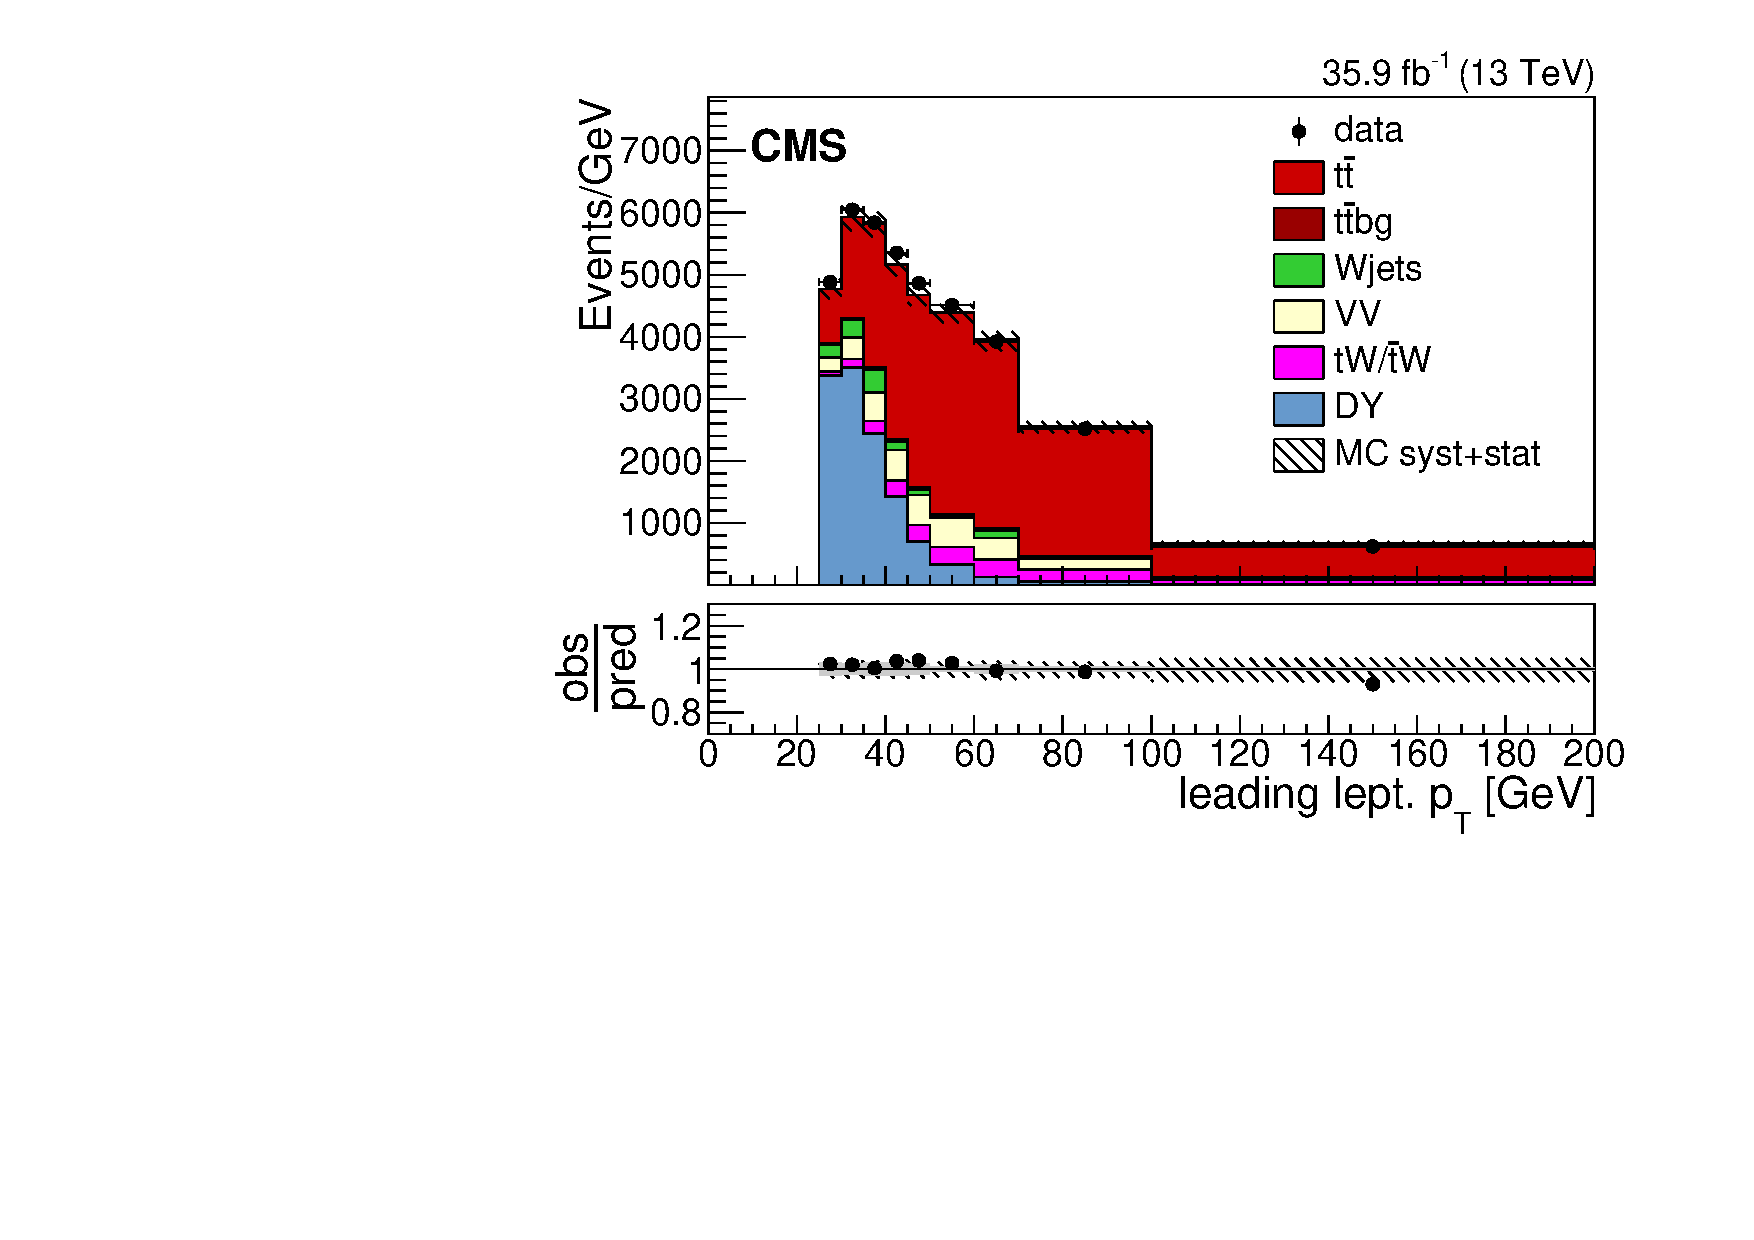
\includegraphics{CrossSection/Figures/ControlPlots/emu_sysnom/lead_lepton_pt_step_8.pdf}}
    \resizebox{0.48 \textwidth}{!}{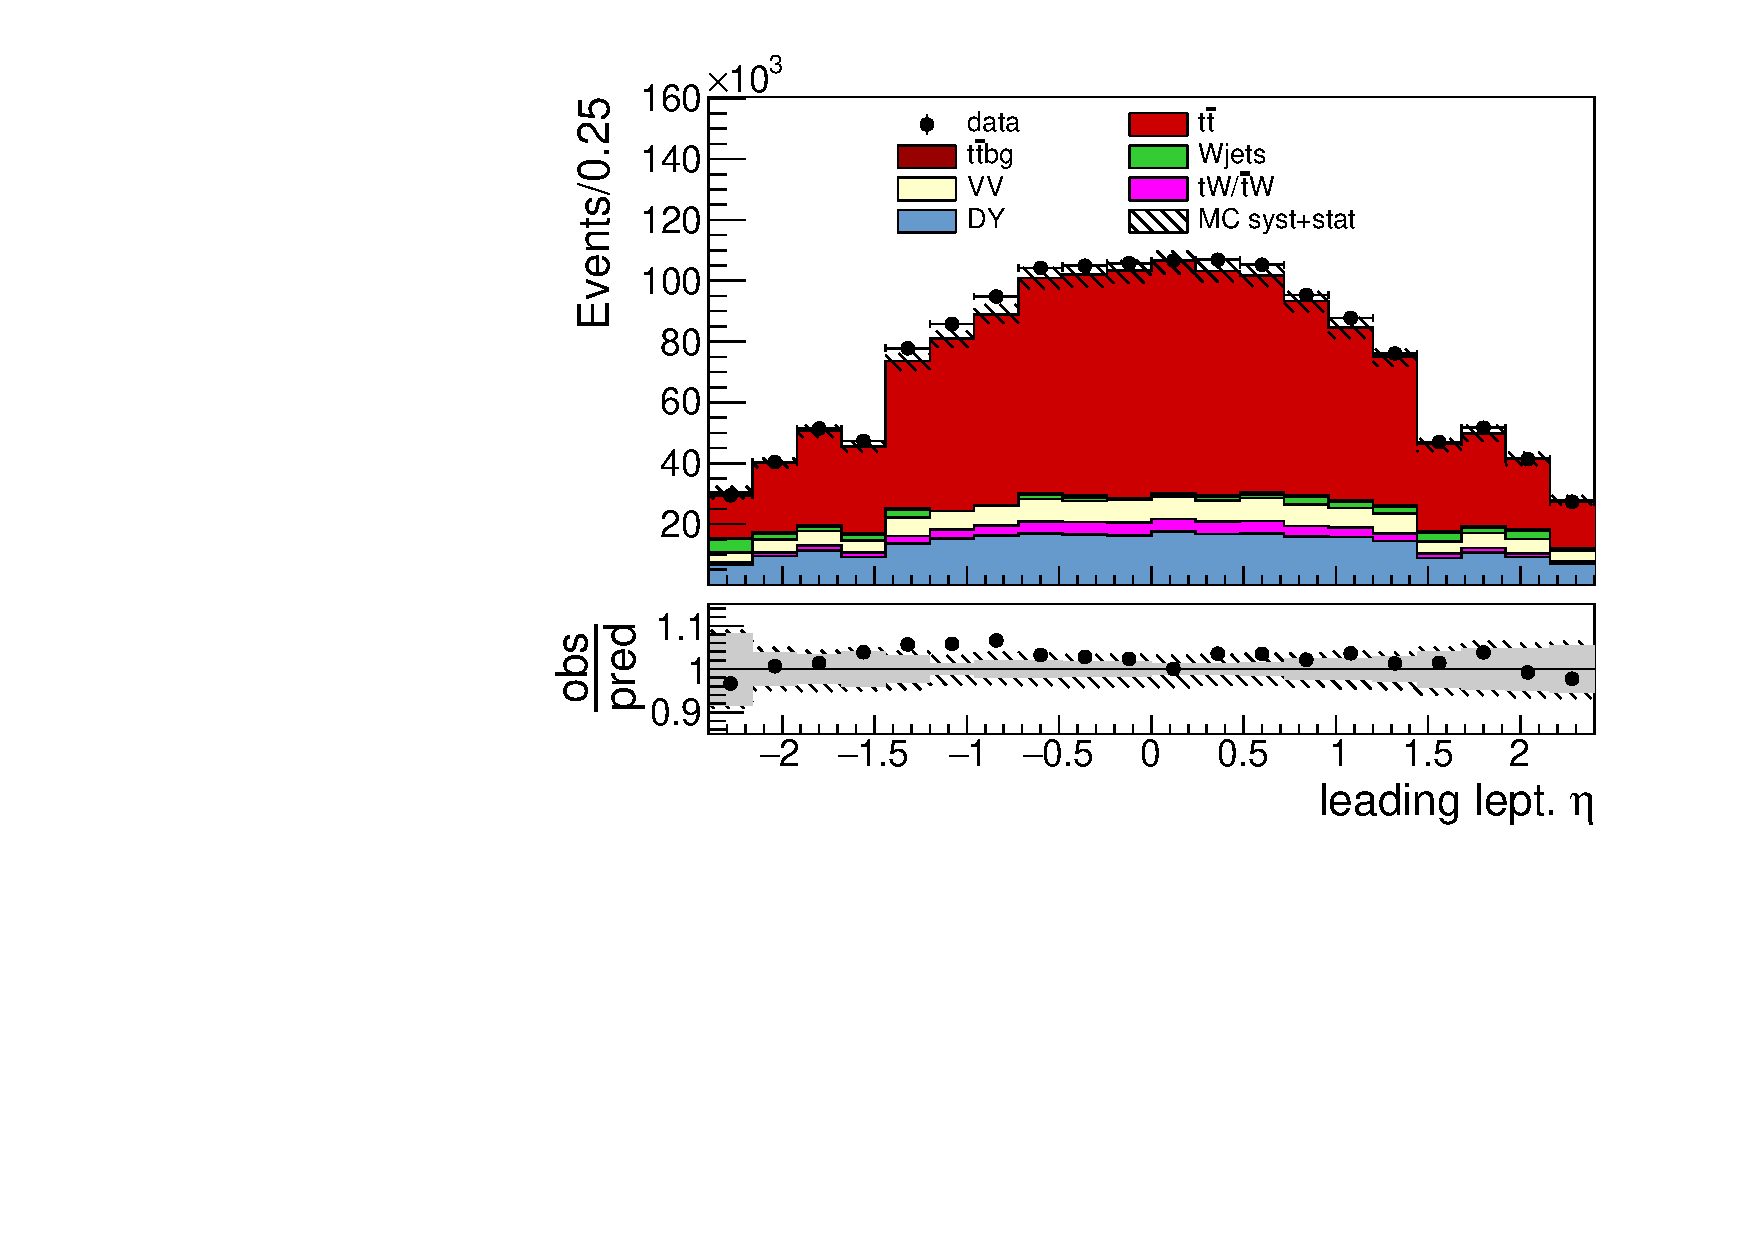
\includegraphics{CrossSection/Figures/ControlPlots/emu_sysnom/lead_lepton_eta_step_8.pdf}}
    \resizebox{0.48 \textwidth}{!}{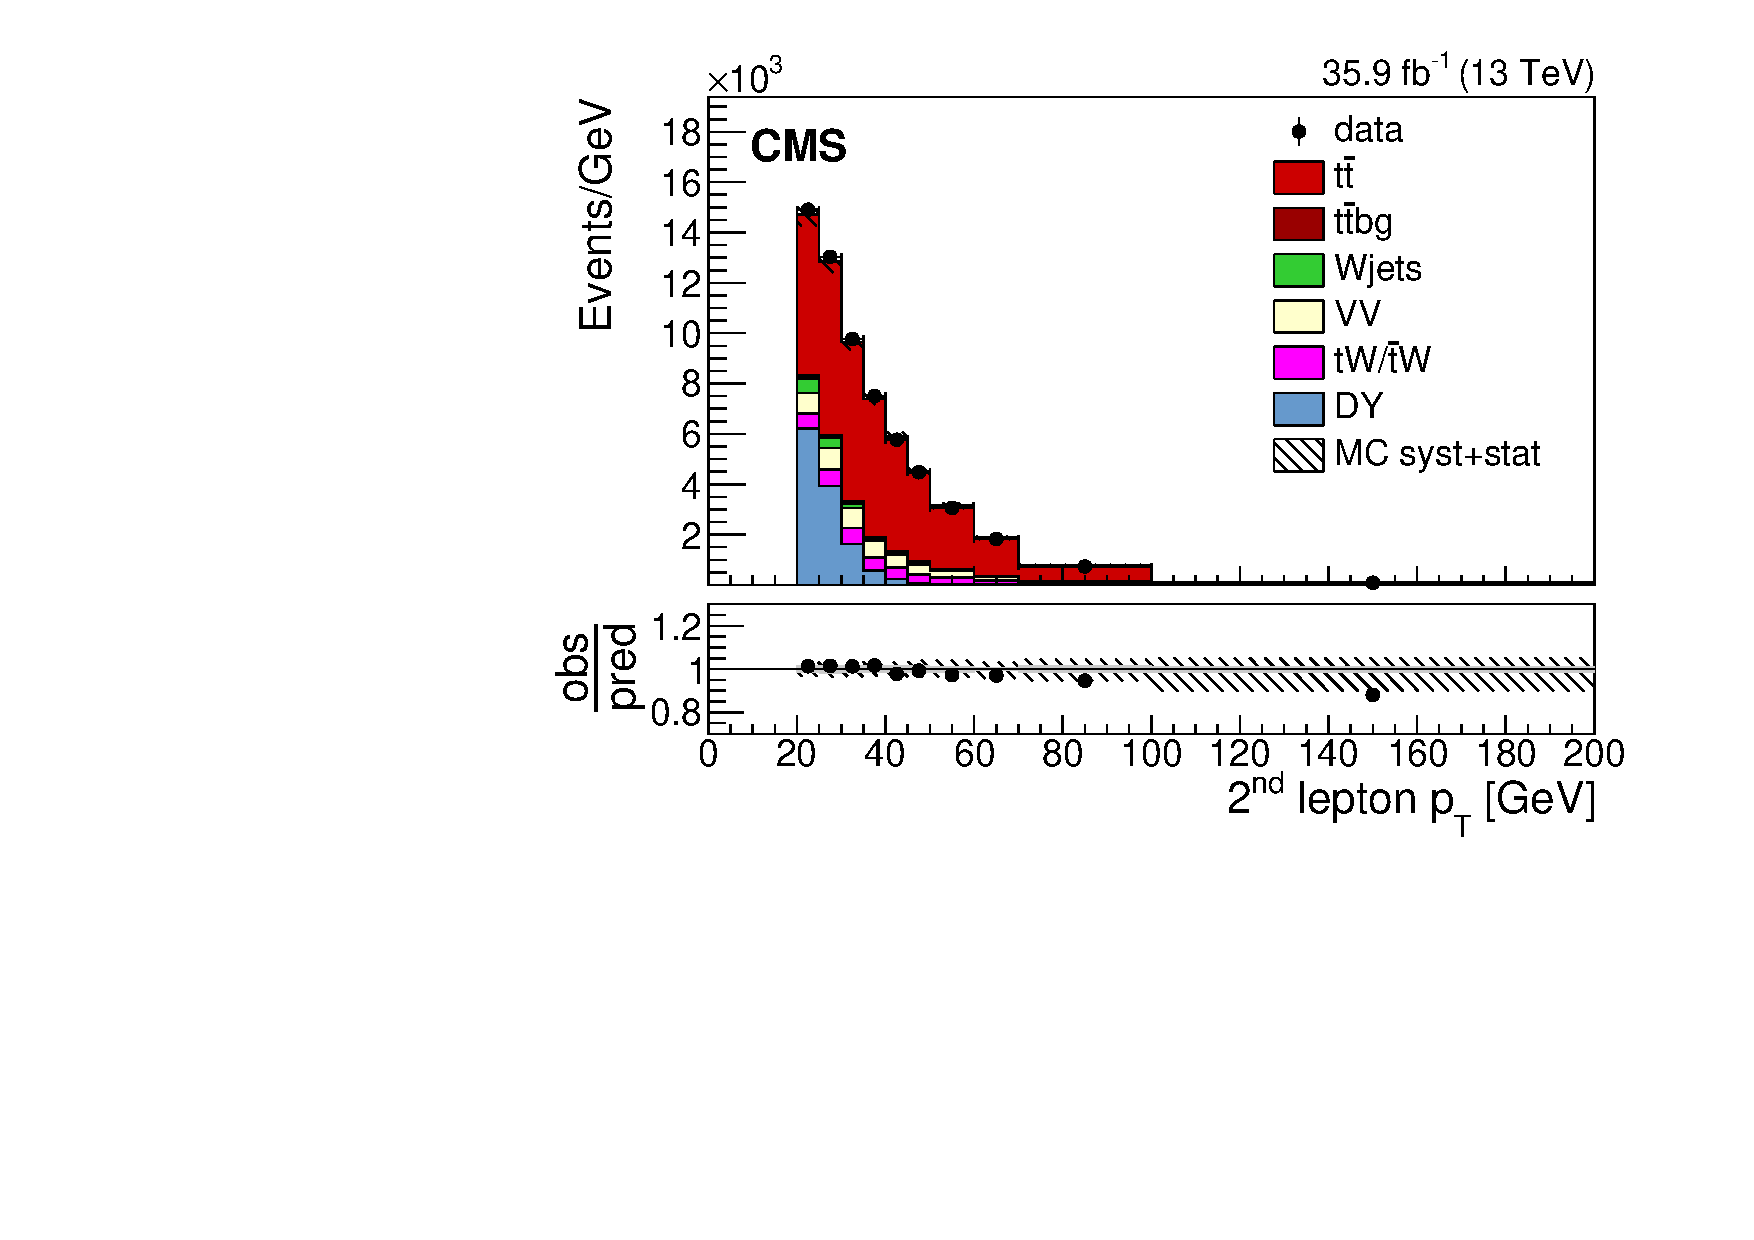
\includegraphics{CrossSection/Figures/ControlPlots/emu_sysnom/seclead_lepton_pt_step_8.pdf}}
    \resizebox{0.48 \textwidth}{!}{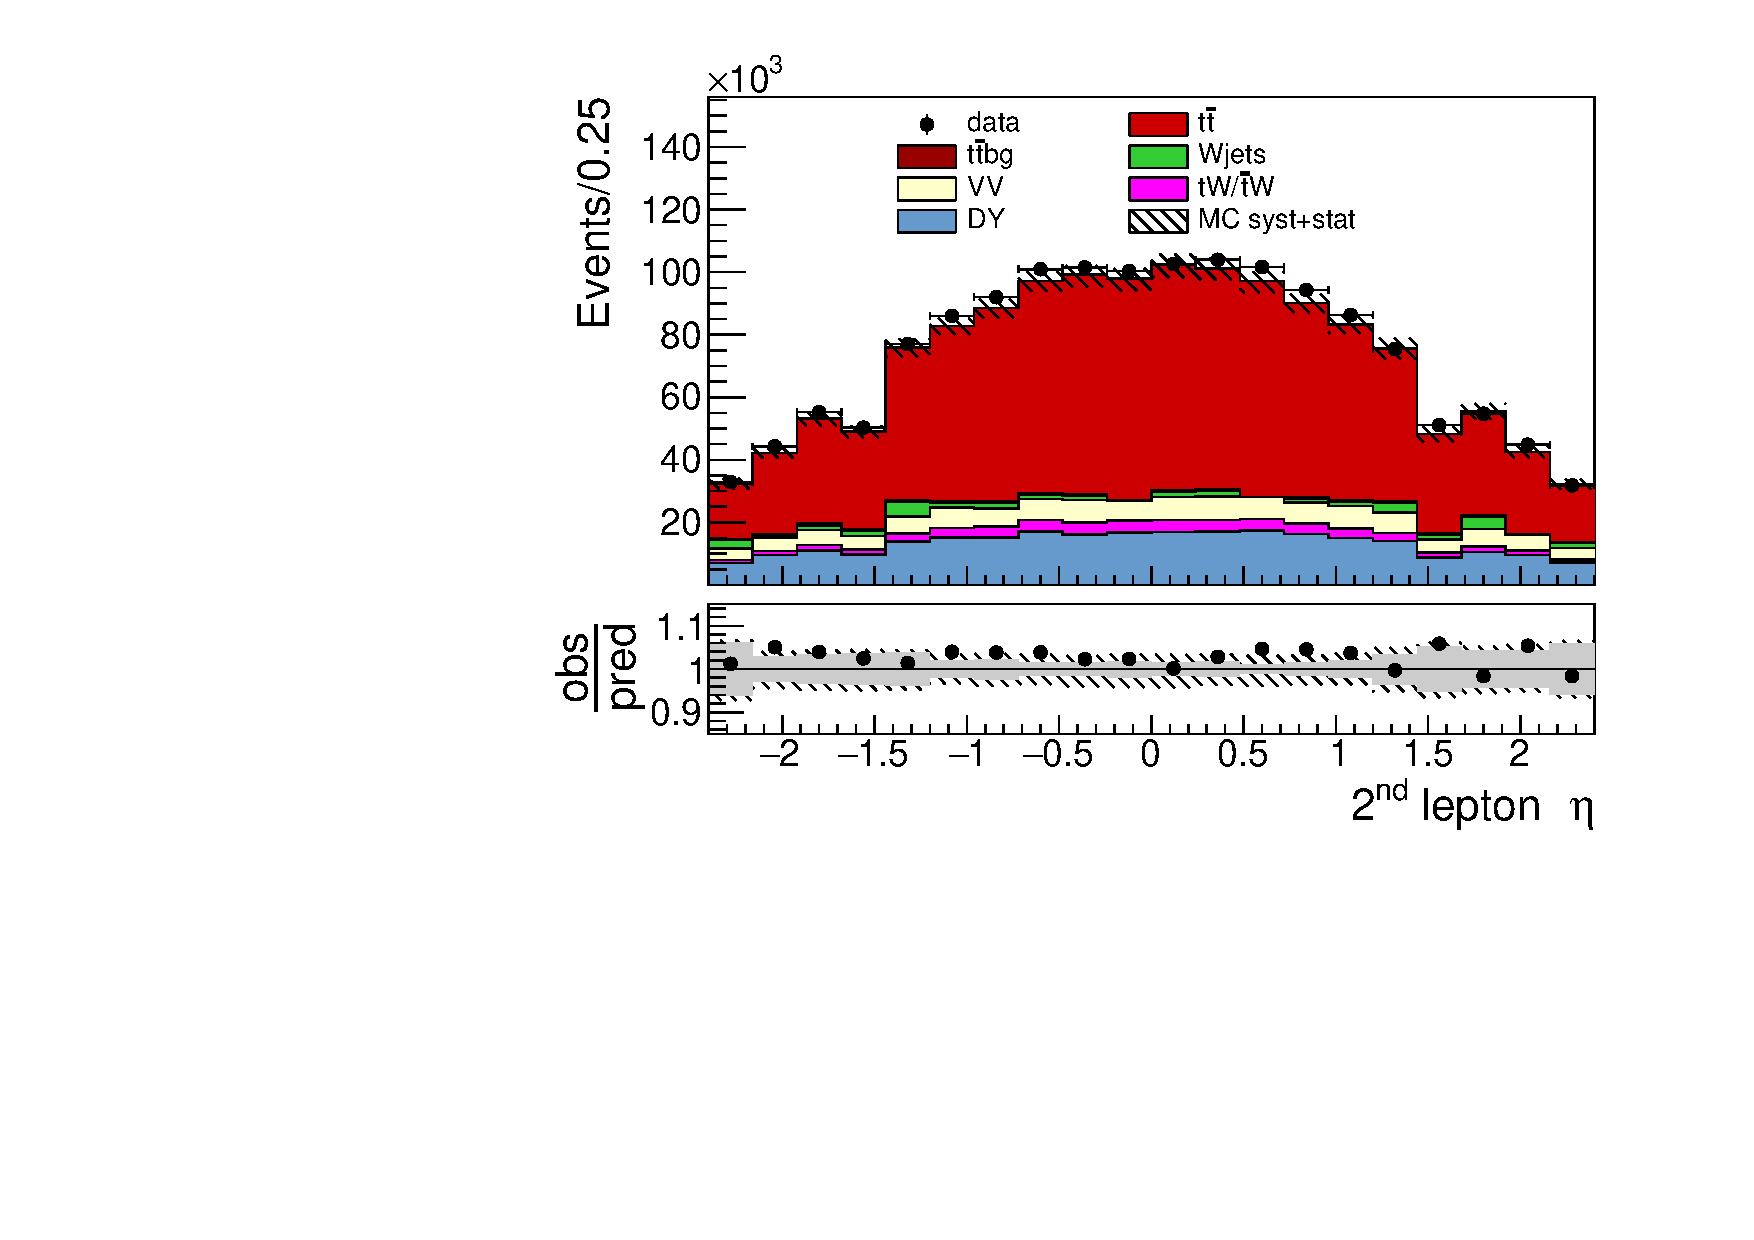
\includegraphics{CrossSection/Figures/ControlPlots/emu_sysnom/seclead_lepton_eta_step_8.pdf}}
    \resizebox{0.48 \textwidth}{!}{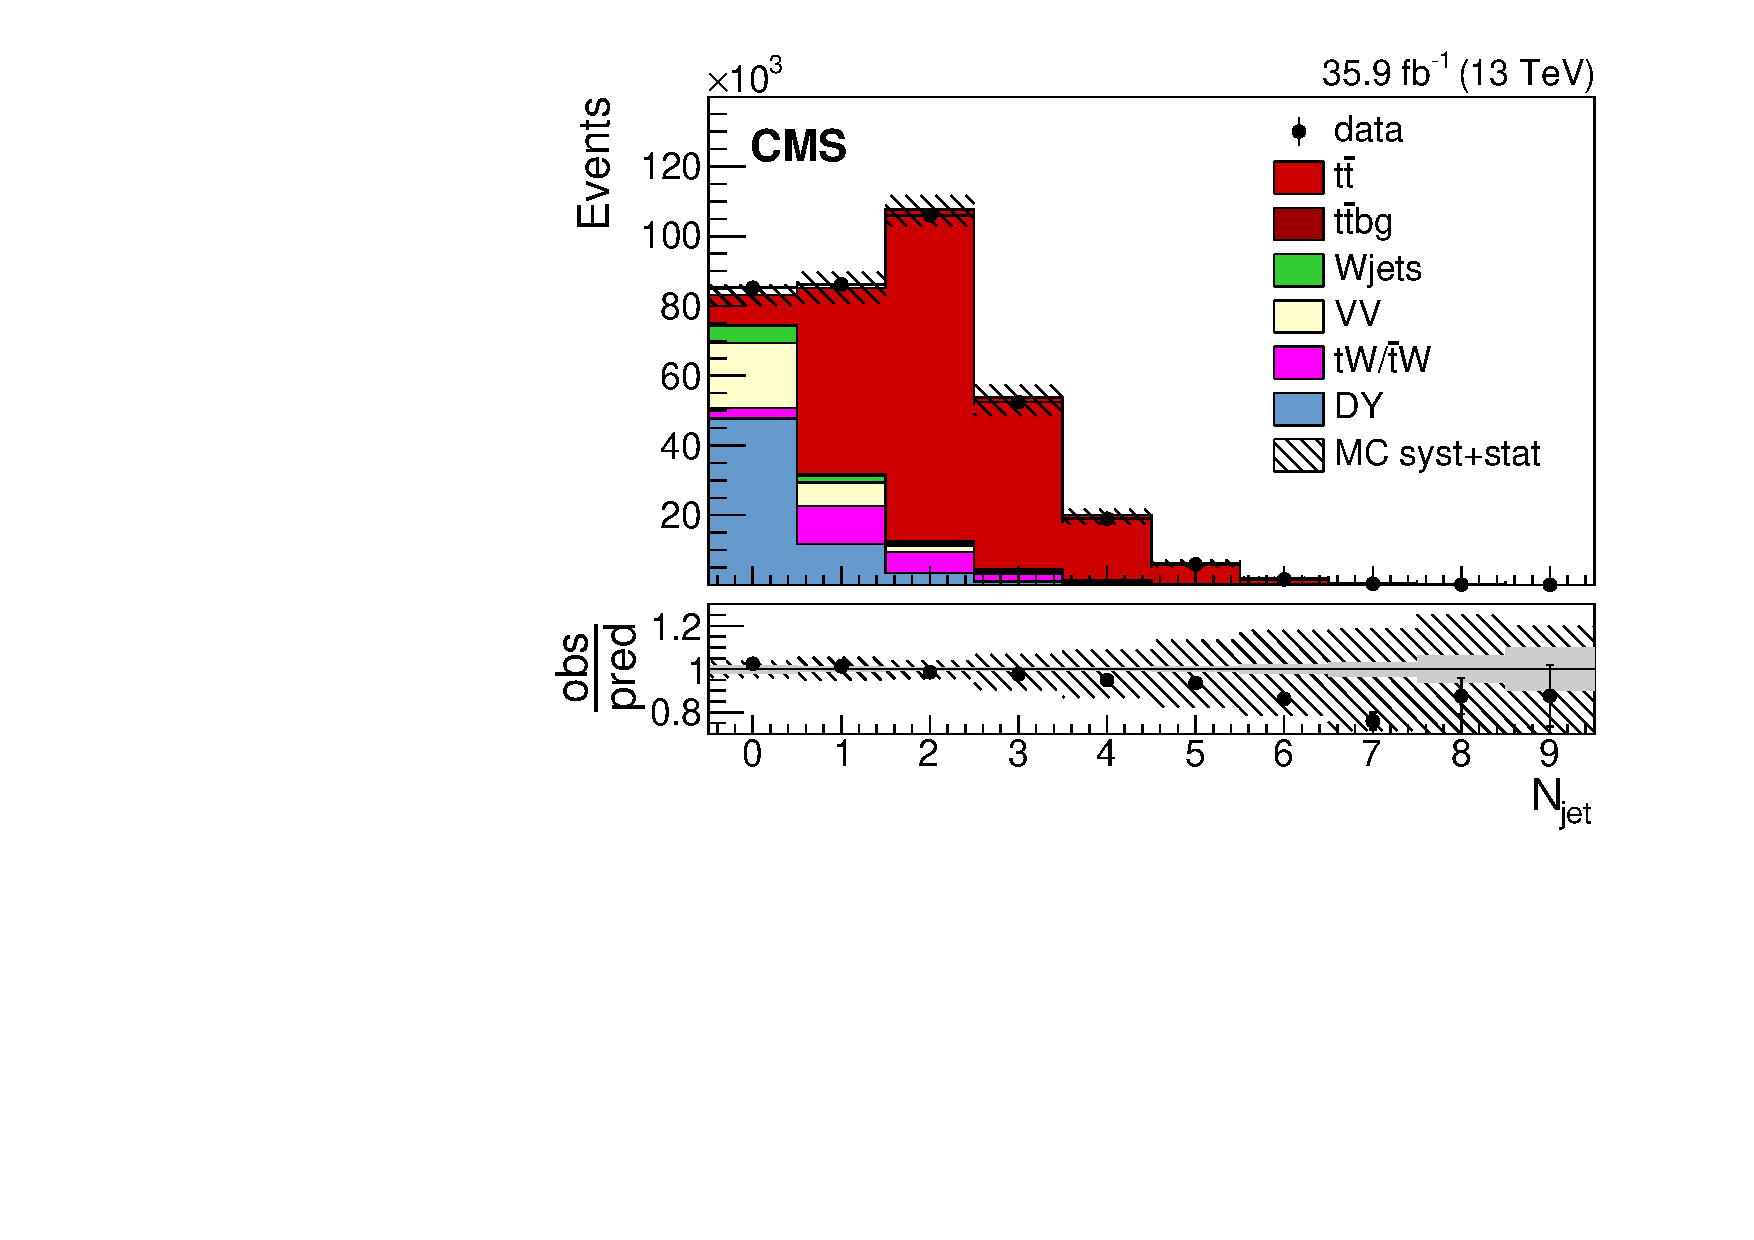
\includegraphics{CrossSection/Figures/ControlPlots/emu_sysnom/selected_jets_multi_step_8.pdf}}
    \resizebox{0.48 \textwidth}{!}{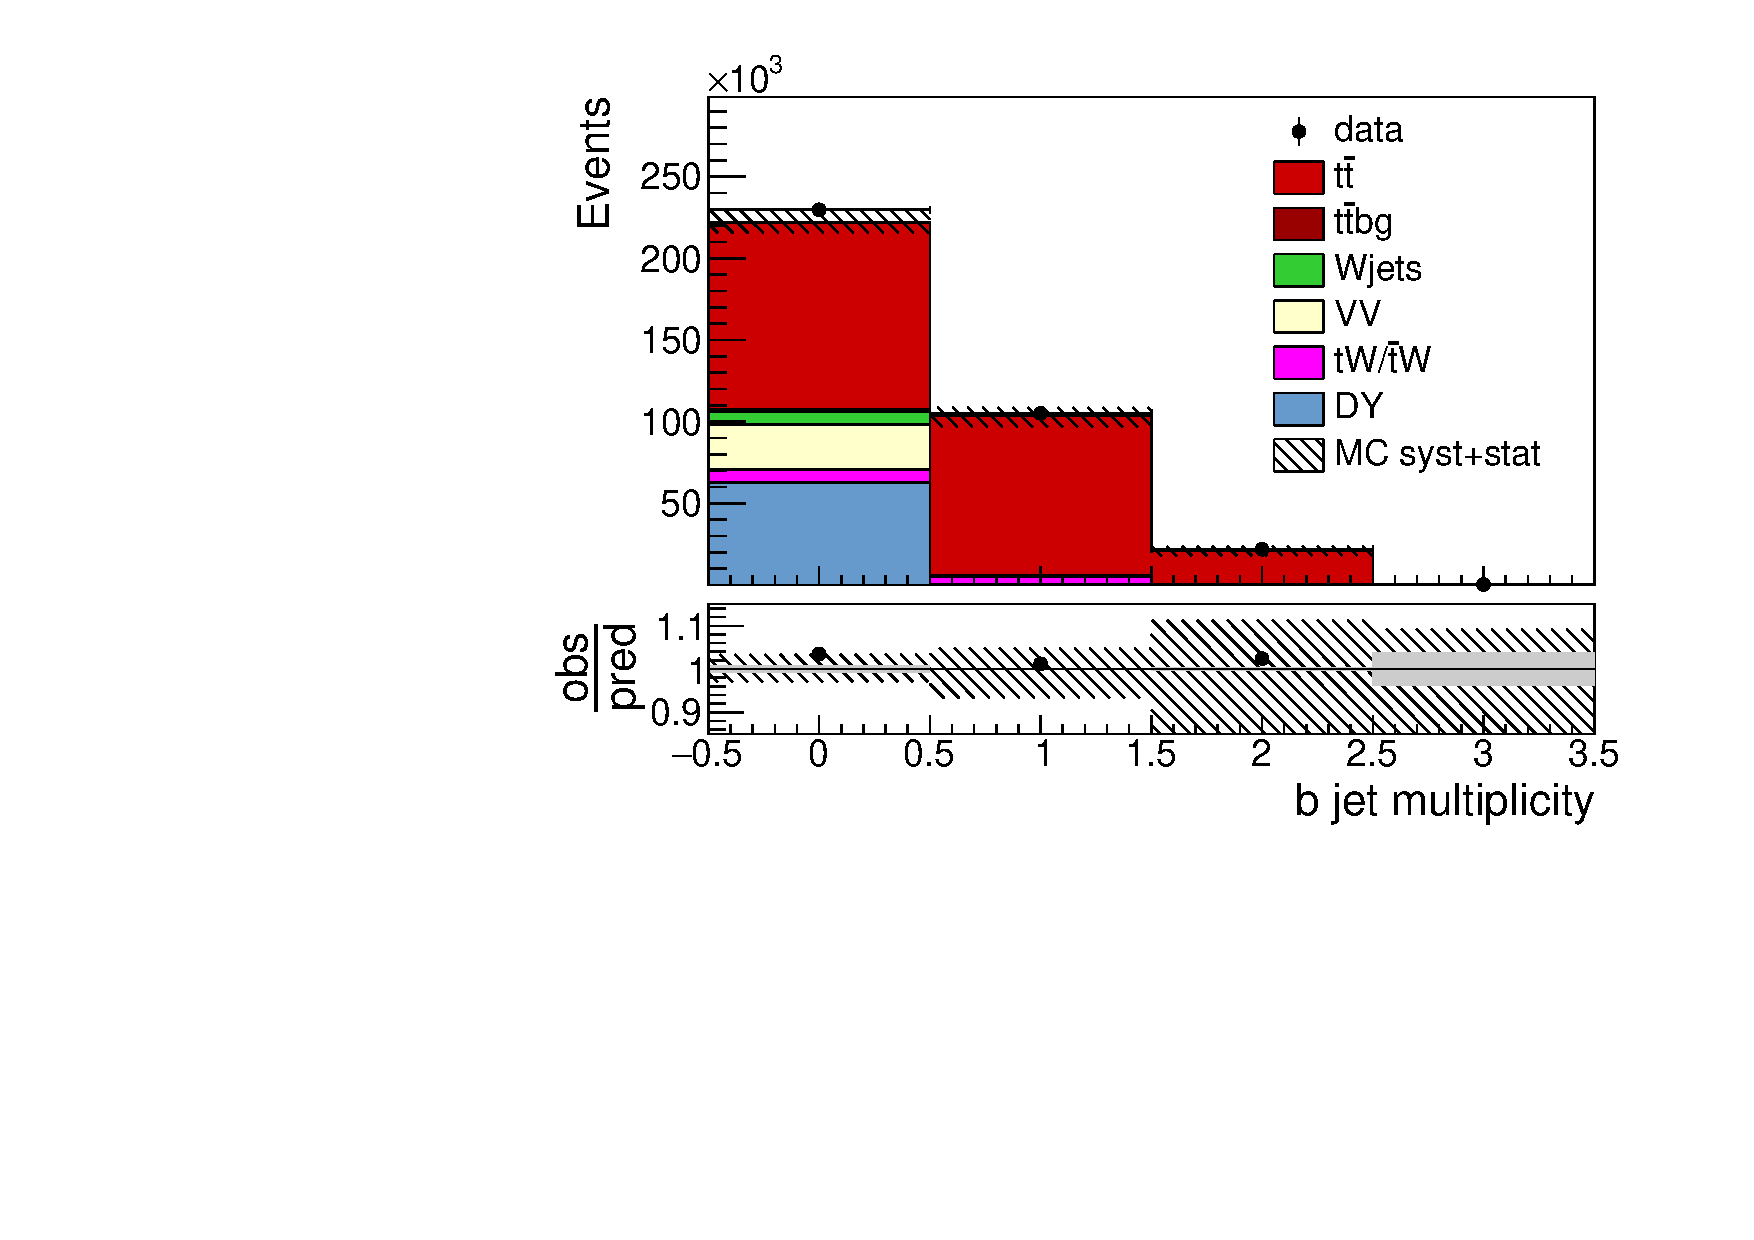
\includegraphics{CrossSection/Figures/ControlPlots/emu_sysnom/selected_b-jet_multi_step_8.pdf}}
      \caption{Transverse momentum (left) and pseudorapidity (right)
        of leading (first row) and second-leading (second row) lepton in the \emu channel after the
        event selection required by the \ttbar cross section
        extraction technique based on a simultaneous fit.
        Jet and b-jet multiplicity after the same selection steps are
        shown in the third row. The hatched
        bands correspond to the total uncertainty on the sum of the
        predicted yields. 
        %agrohsje , excluding luminosity and background
        %normalization uncertainties. 
        The ratios of data to the sum of the predicted yields are
        shown at the bottom of each plot. Here, the solid gray band
        represents the contribution of the statistical uncertainty.}  
       \label{fig:xsec_emu_ctrplots}
  \end{center}
\end{figure}

\begin{figure}[htbp!]
  \begin{center}
    \resizebox{0.48 \textwidth}{!}{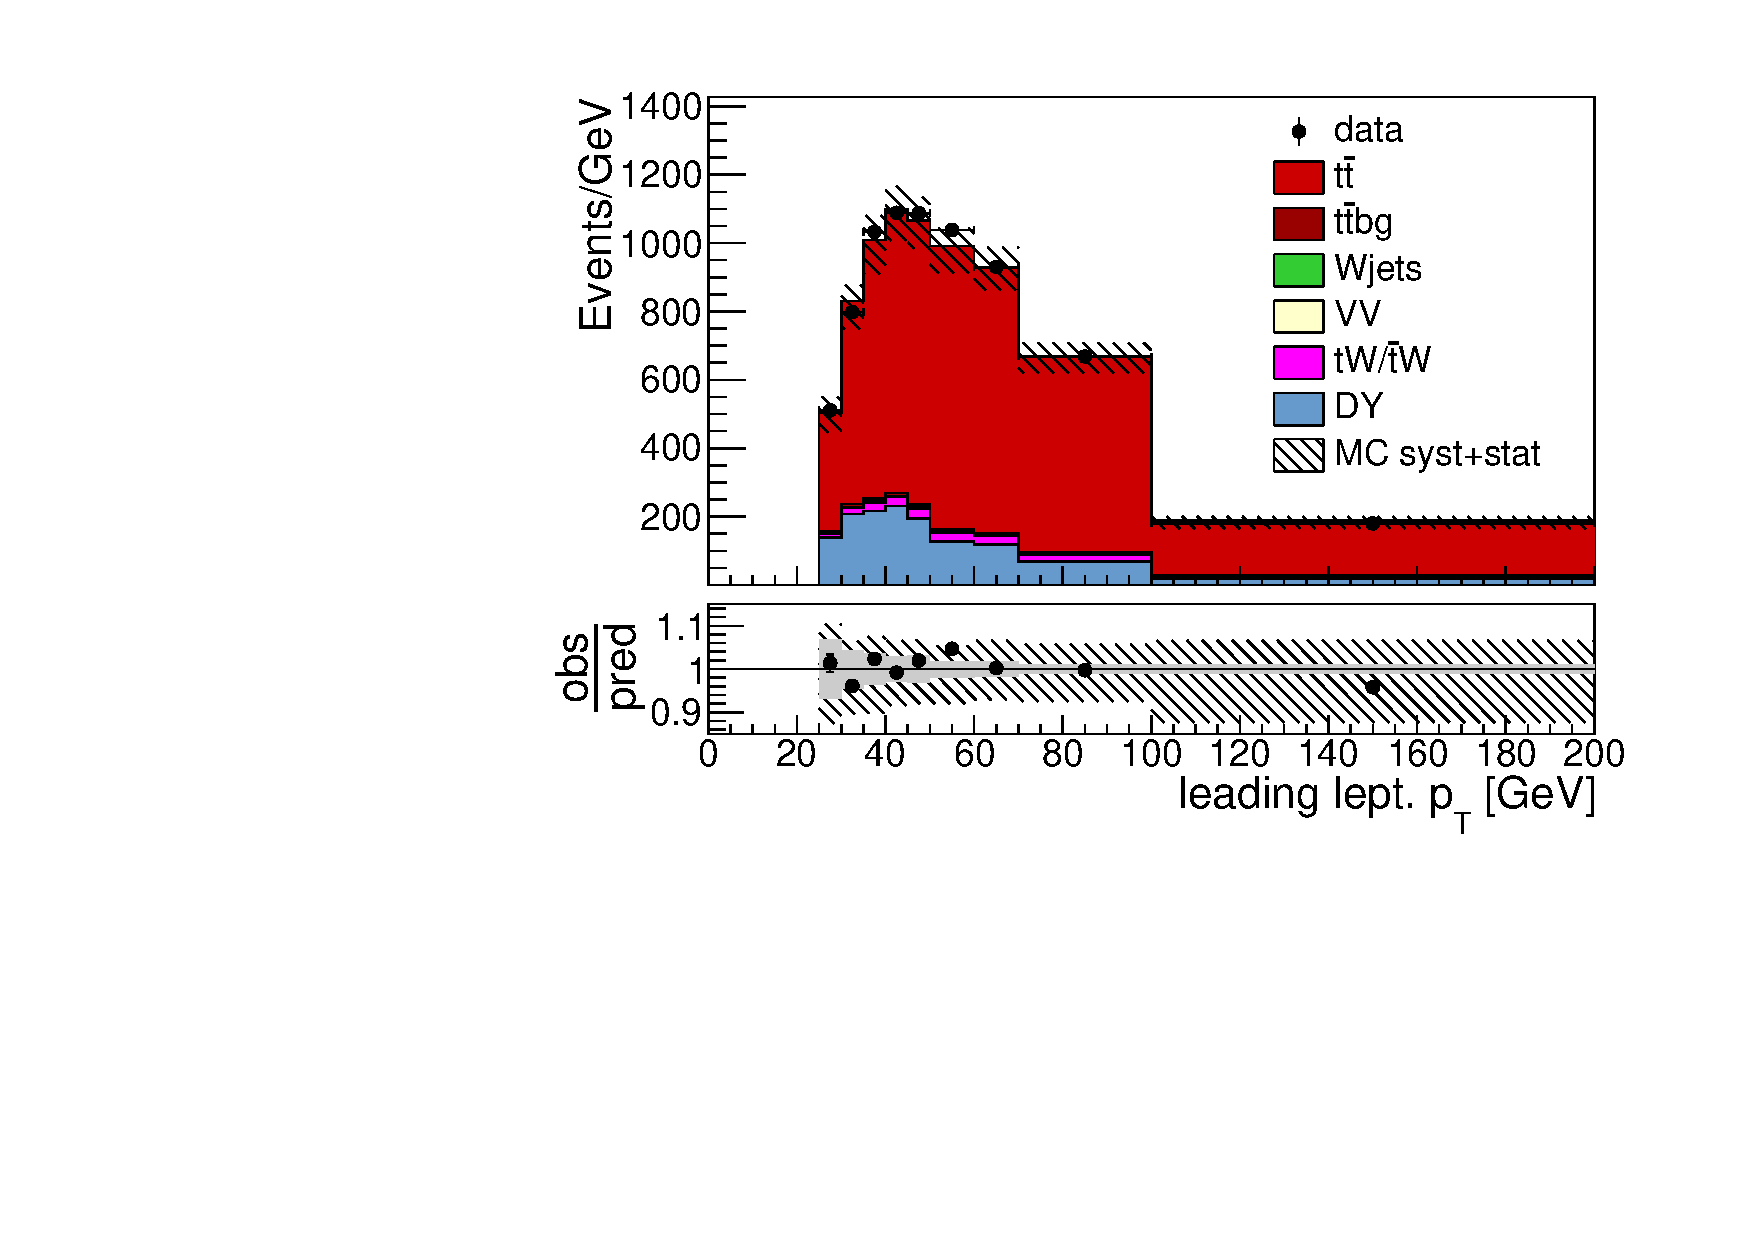
\includegraphics{CrossSection/Figures/ControlPlots/mumu_sysnom/lead_lepton_pt_step_8.pdf}}
    \resizebox{0.48 \textwidth}{!}{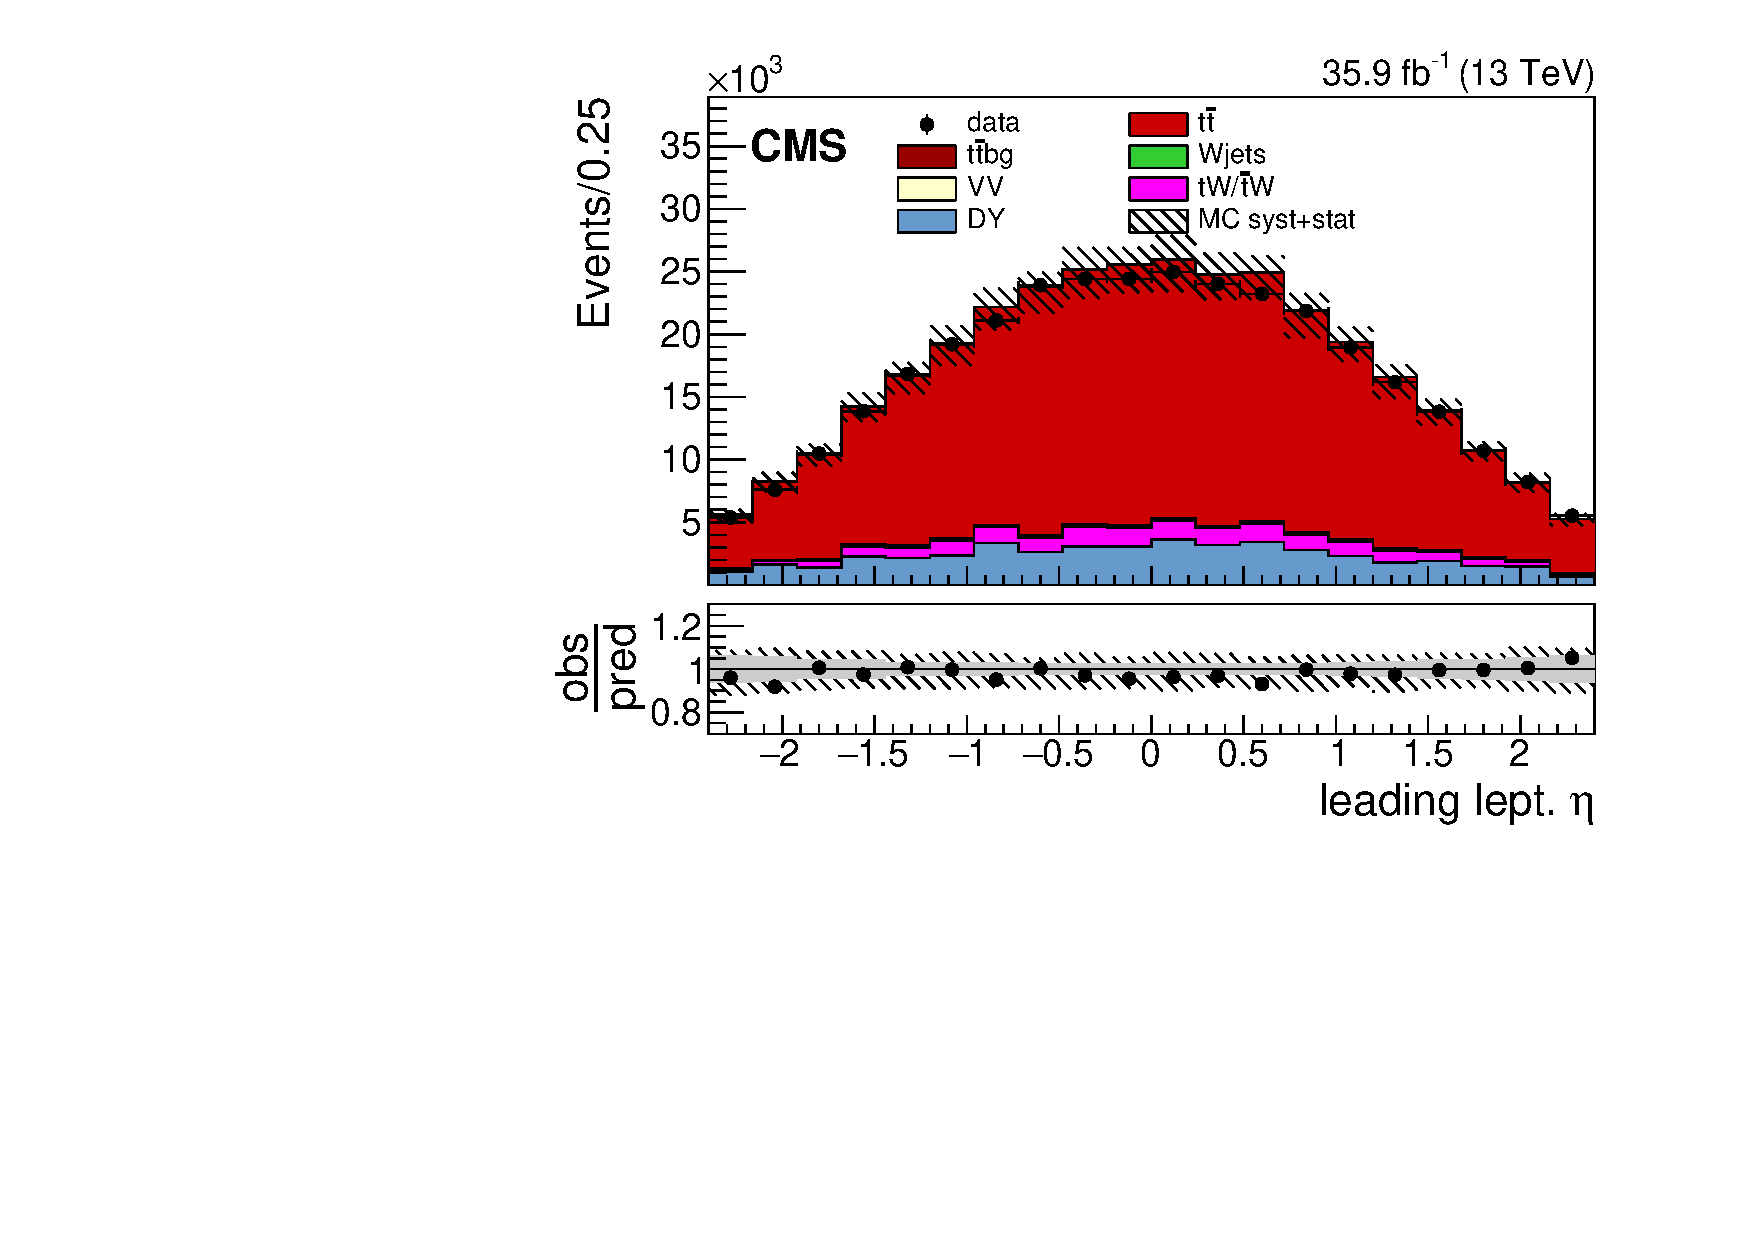
\includegraphics{CrossSection/Figures/ControlPlots/mumu_sysnom/lead_lepton_eta_step_8.pdf}}
    \resizebox{0.48 \textwidth}{!}{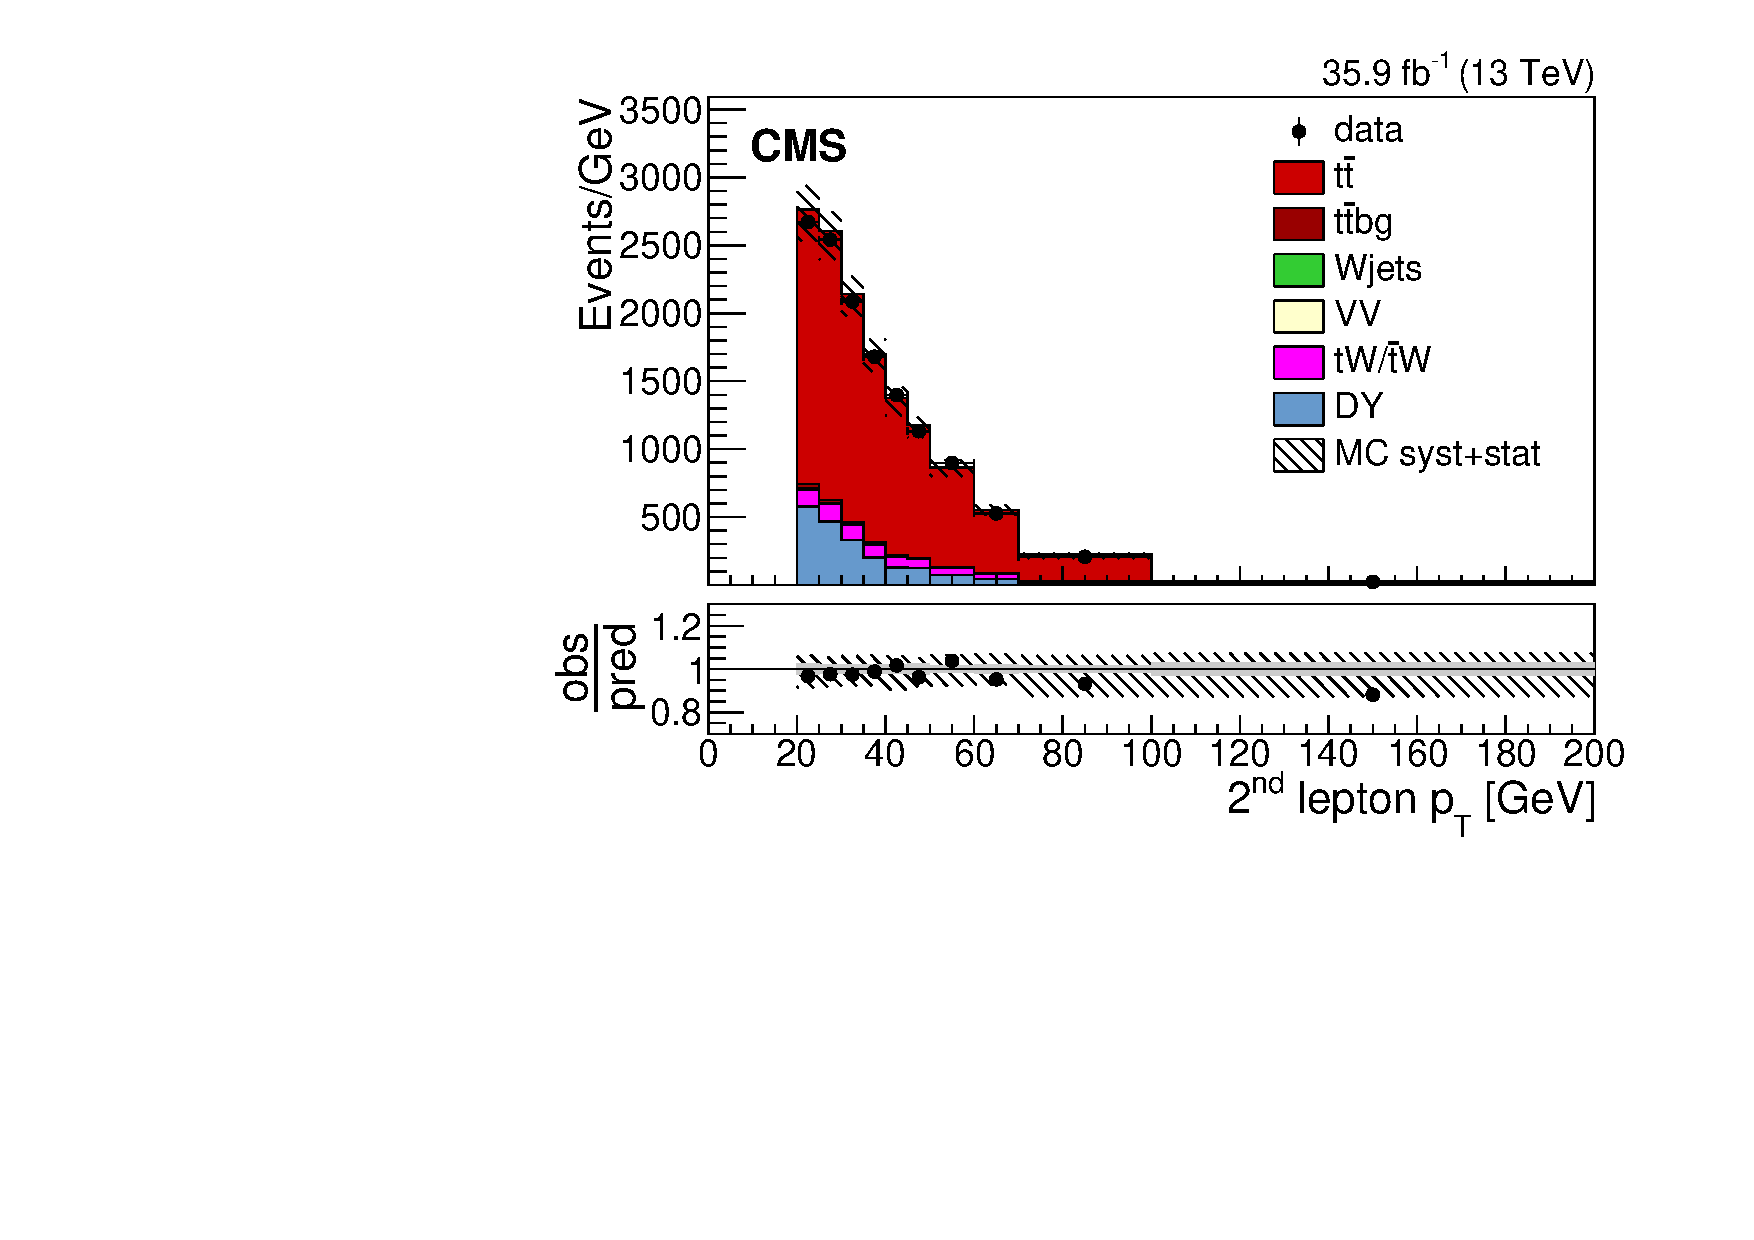
\includegraphics{CrossSection/Figures/ControlPlots/mumu_sysnom/seclead_lepton_pt_step_8.pdf}}
    \resizebox{0.48 \textwidth}{!}{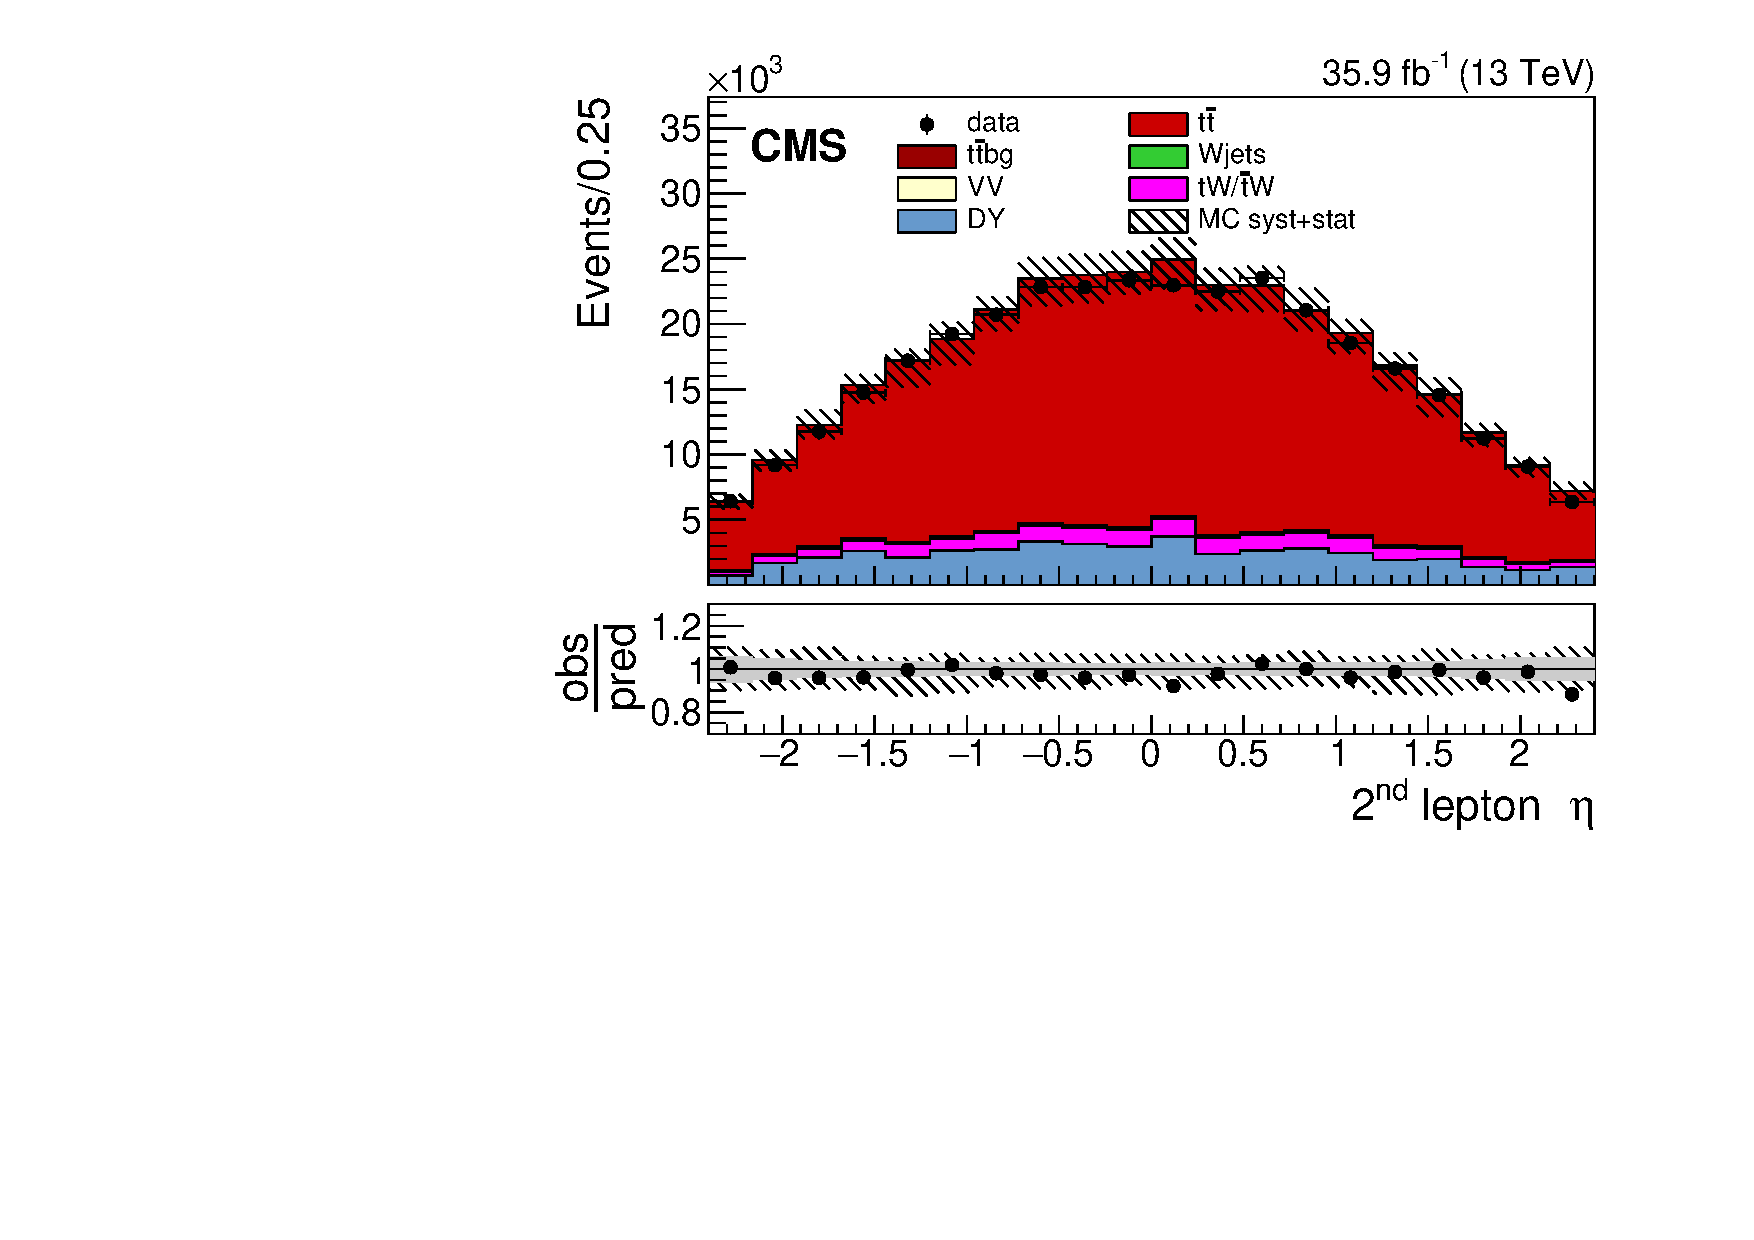
\includegraphics{CrossSection/Figures/ControlPlots/mumu_sysnom/seclead_lepton_eta_step_8.pdf}}
    \resizebox{0.48 \textwidth}{!}{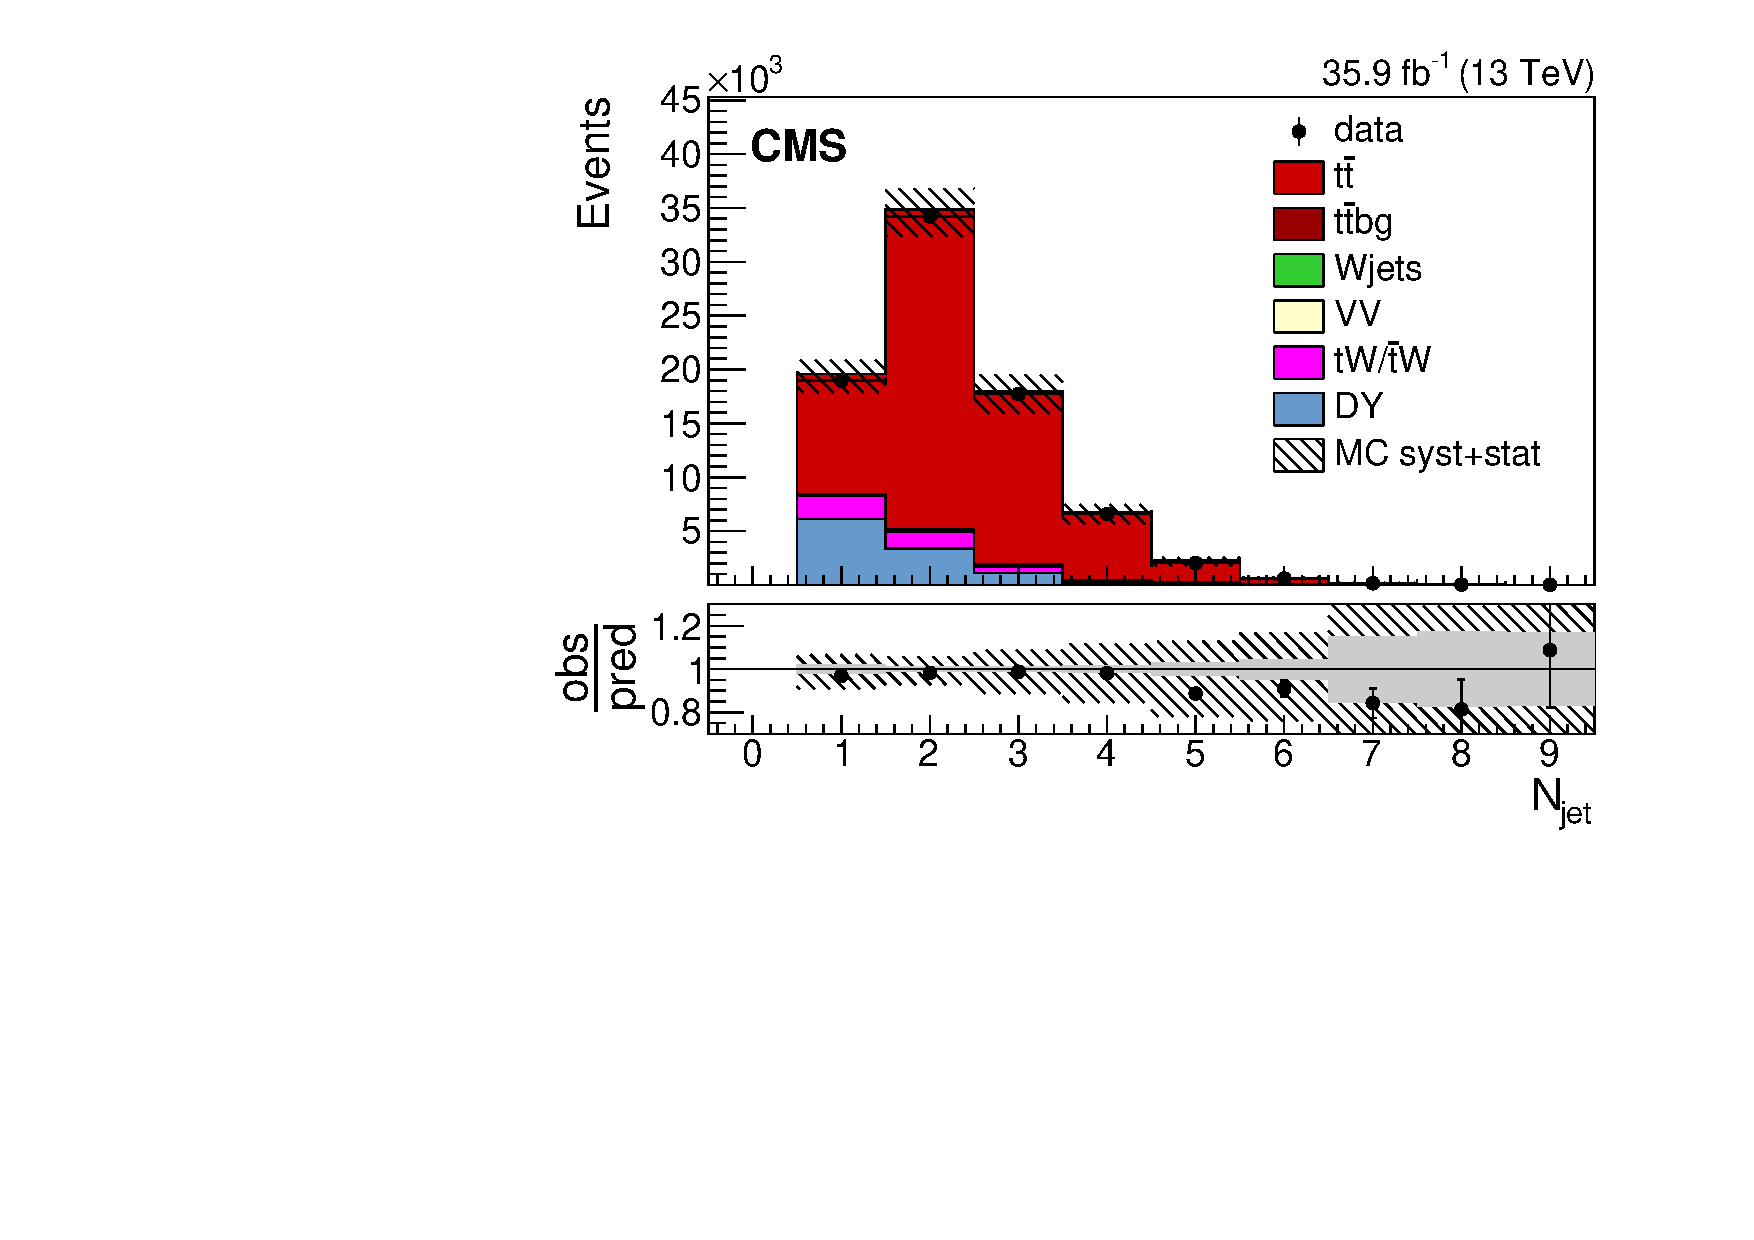
\includegraphics{CrossSection/Figures/ControlPlots/mumu_sysnom/selected_jets_multi_step_8.pdf}}
    \resizebox{0.48 \textwidth}{!}{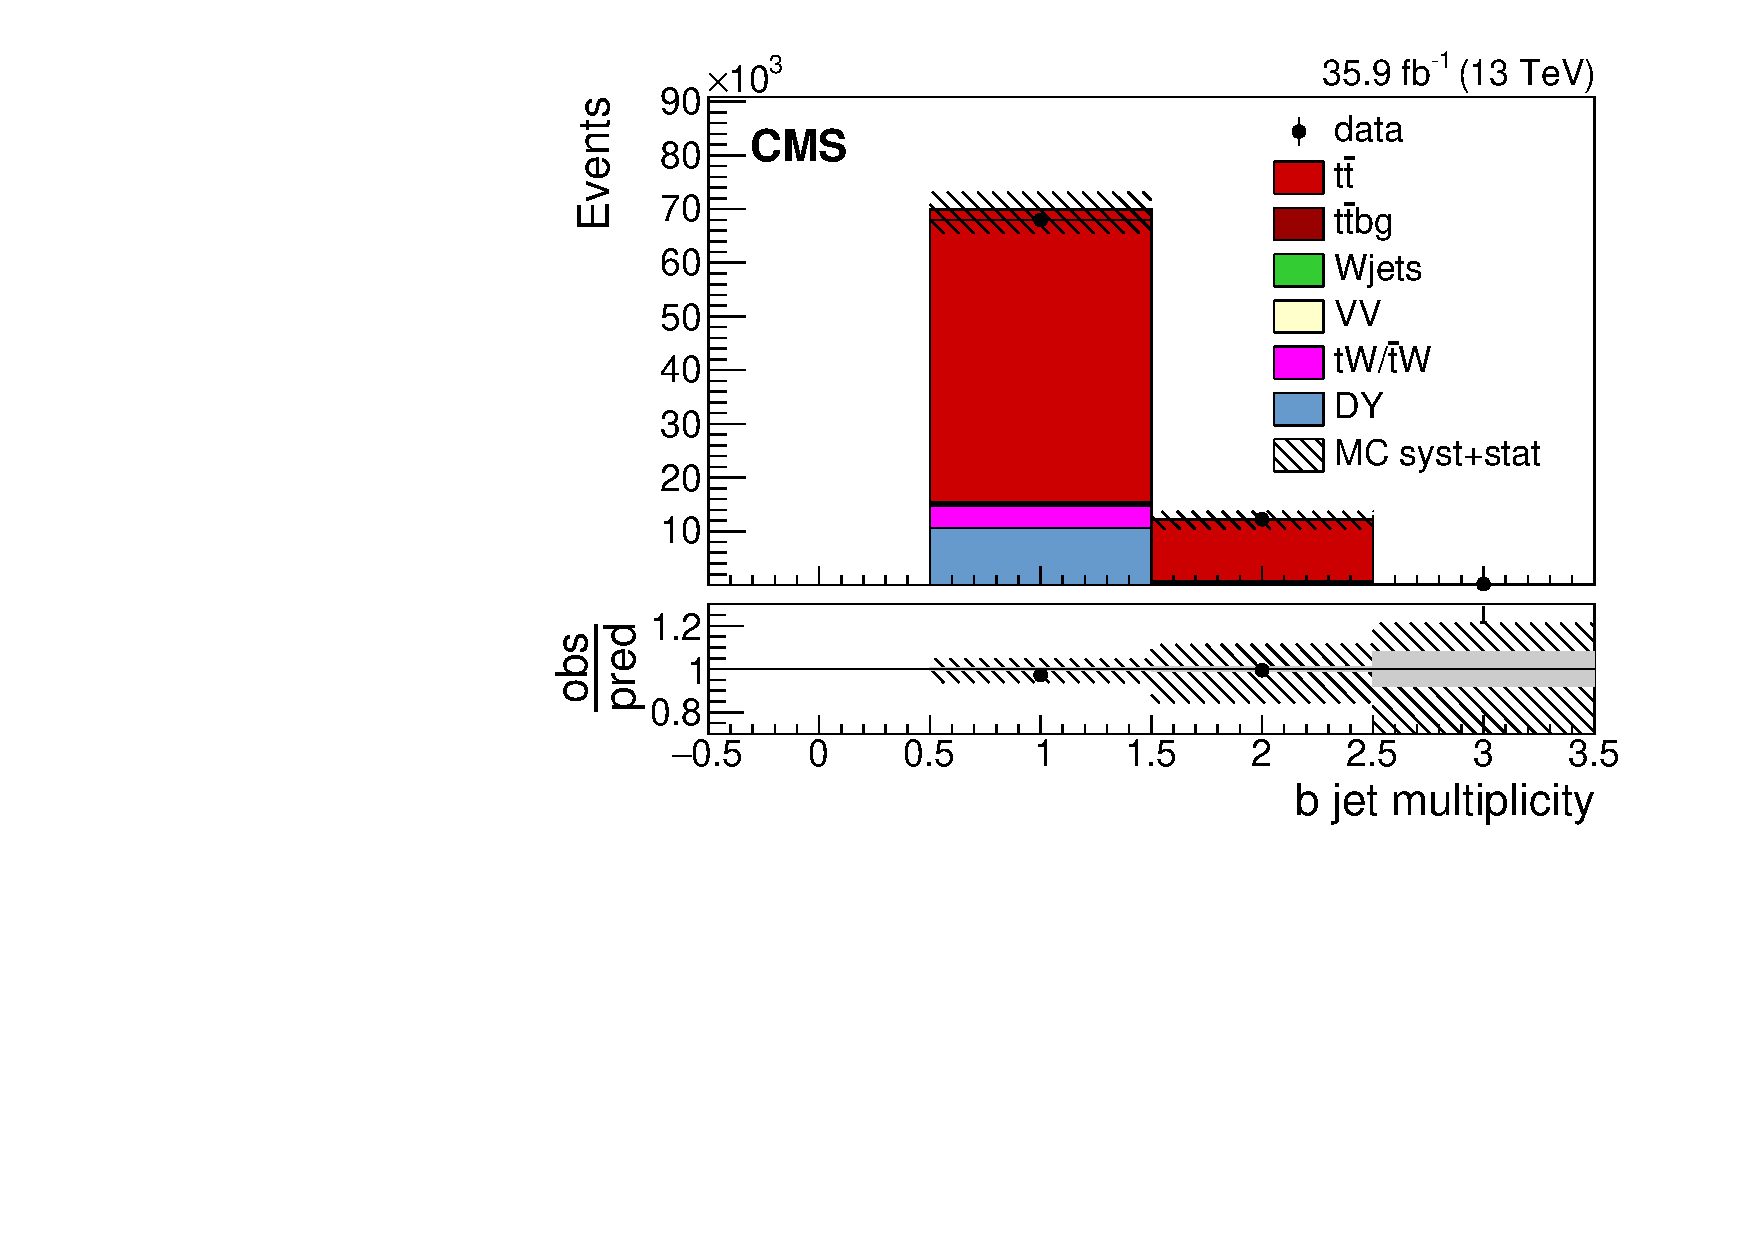
\includegraphics{CrossSection/Figures/ControlPlots/mumu_sysnom/selected_b-jet_multi_step_8.pdf}}
      \caption{Transverse momentum (left) and pseudorapidity (right)
        of leading (first row) and second-leading (second row) lepton in the \mumu channel after the
        event selection required by the \ttbar cross section
        extraction technique based on a simultaneous fit. Jet and b-jet multiplicity after the same selection steps are
        shown in the third row. The hatched
        bands correspond to the total uncertainty on the sum of the
        predicted yields. 
        %agrohsje , excluding luminosity and background
        %normalization uncertainties. 
        The ratios of data to the sum of the predicted yields are
        shown at the bottom of each plot. Here, the solid gray band
        represents the contribution of the statistical uncertainty.}  
       \label{fig:xsec_mumu_ctrplots}
  \end{center}
\end{figure}

\begin{figure}[htbp!]
  \begin{center}
    \resizebox{0.48 \textwidth}{!}{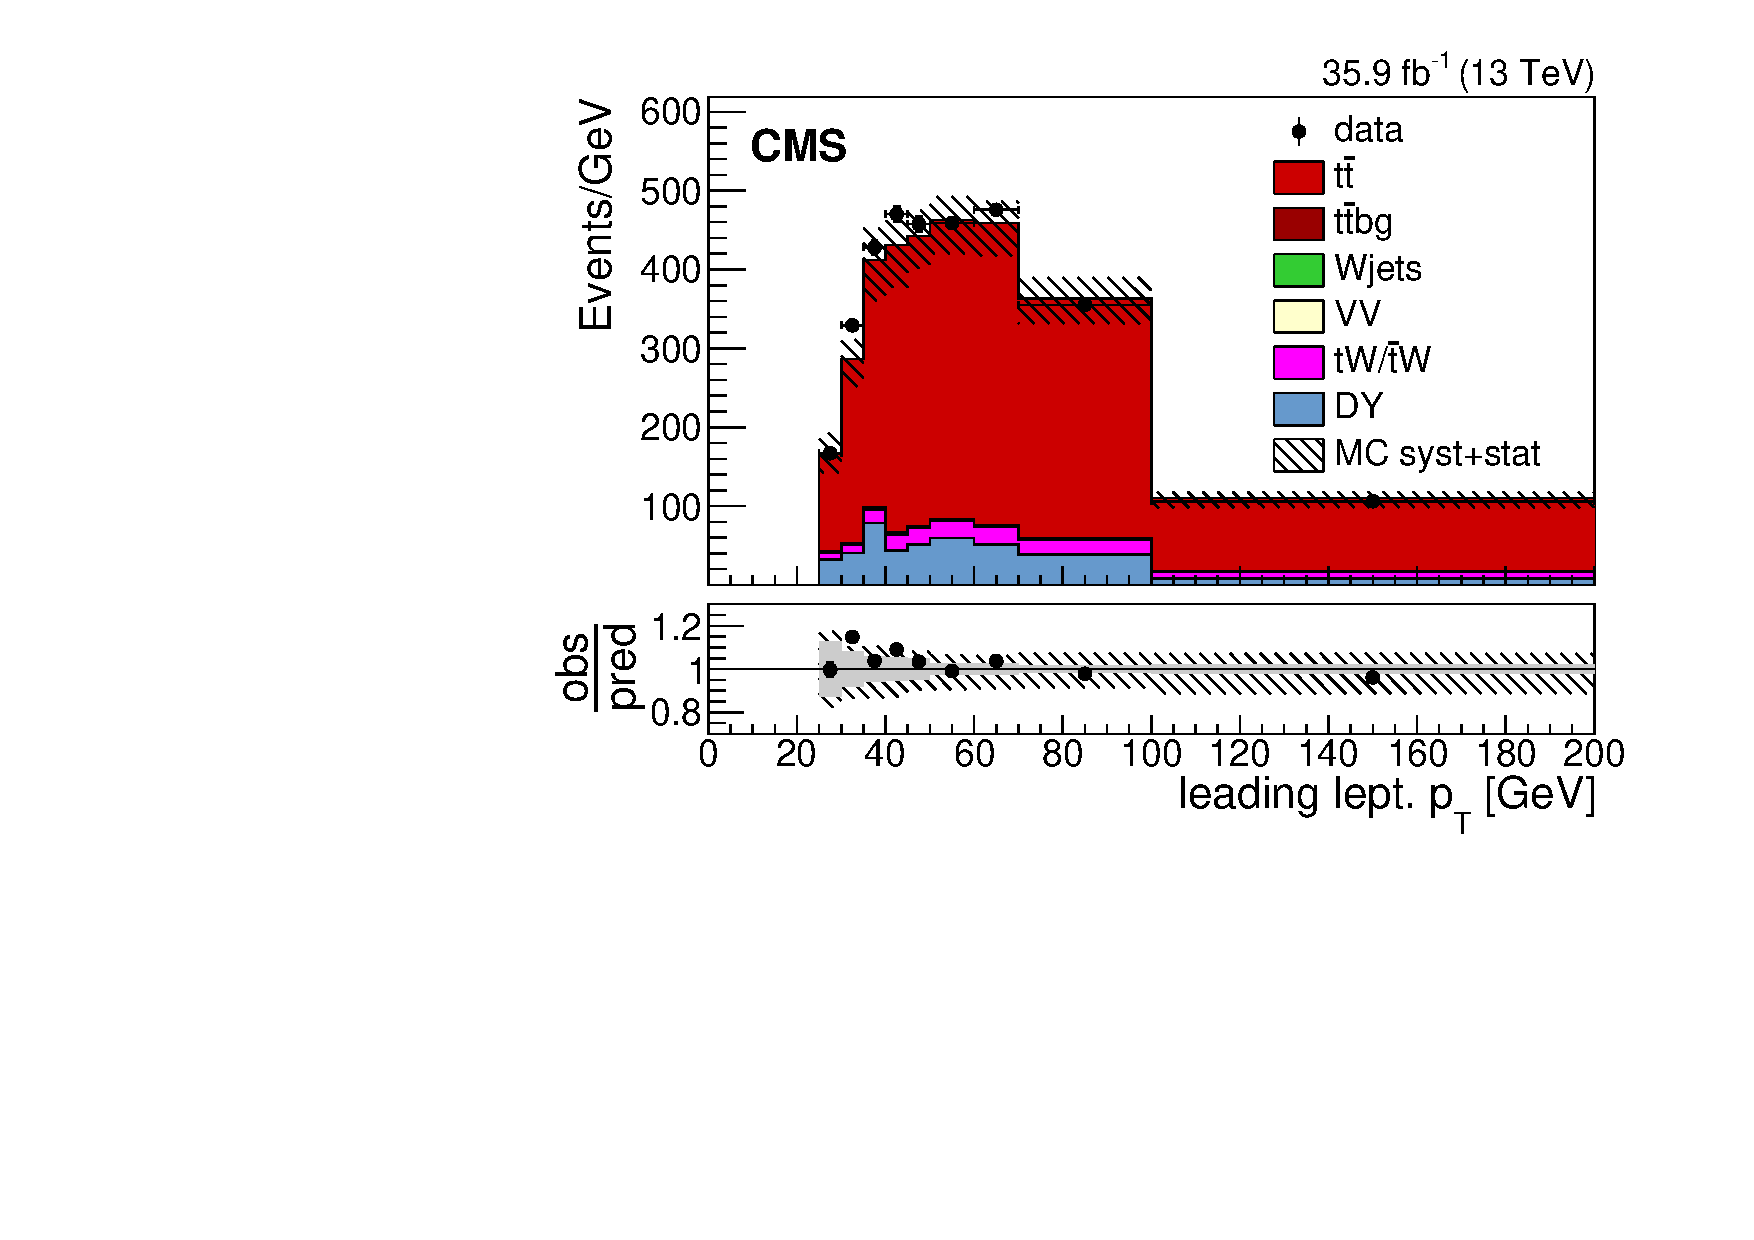
\includegraphics{CrossSection/Figures/ControlPlots/ee_sysnom/lead_lepton_pt_step_8.pdf}}
    \resizebox{0.48 \textwidth}{!}{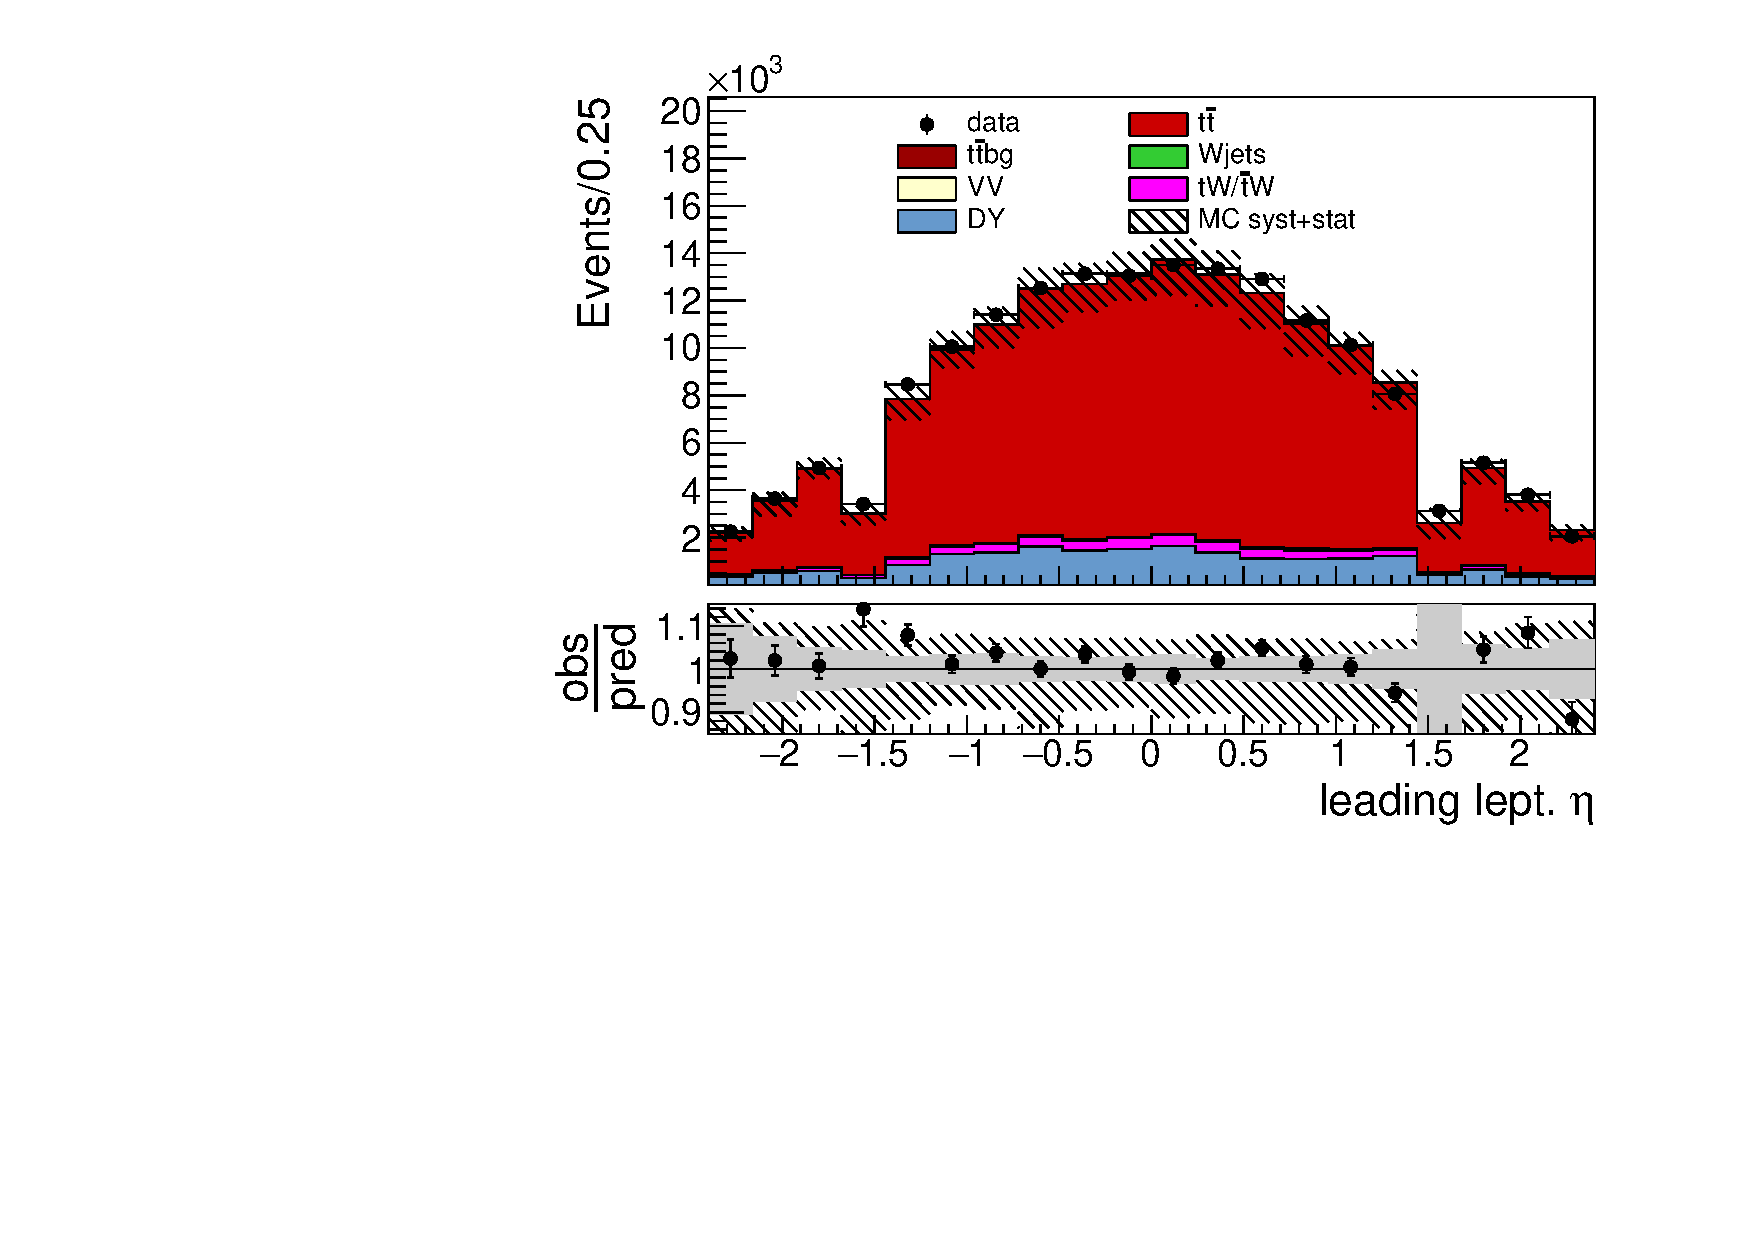
\includegraphics{CrossSection/Figures/ControlPlots/ee_sysnom/lead_lepton_eta_step_8.pdf}}
    \resizebox{0.48 \textwidth}{!}{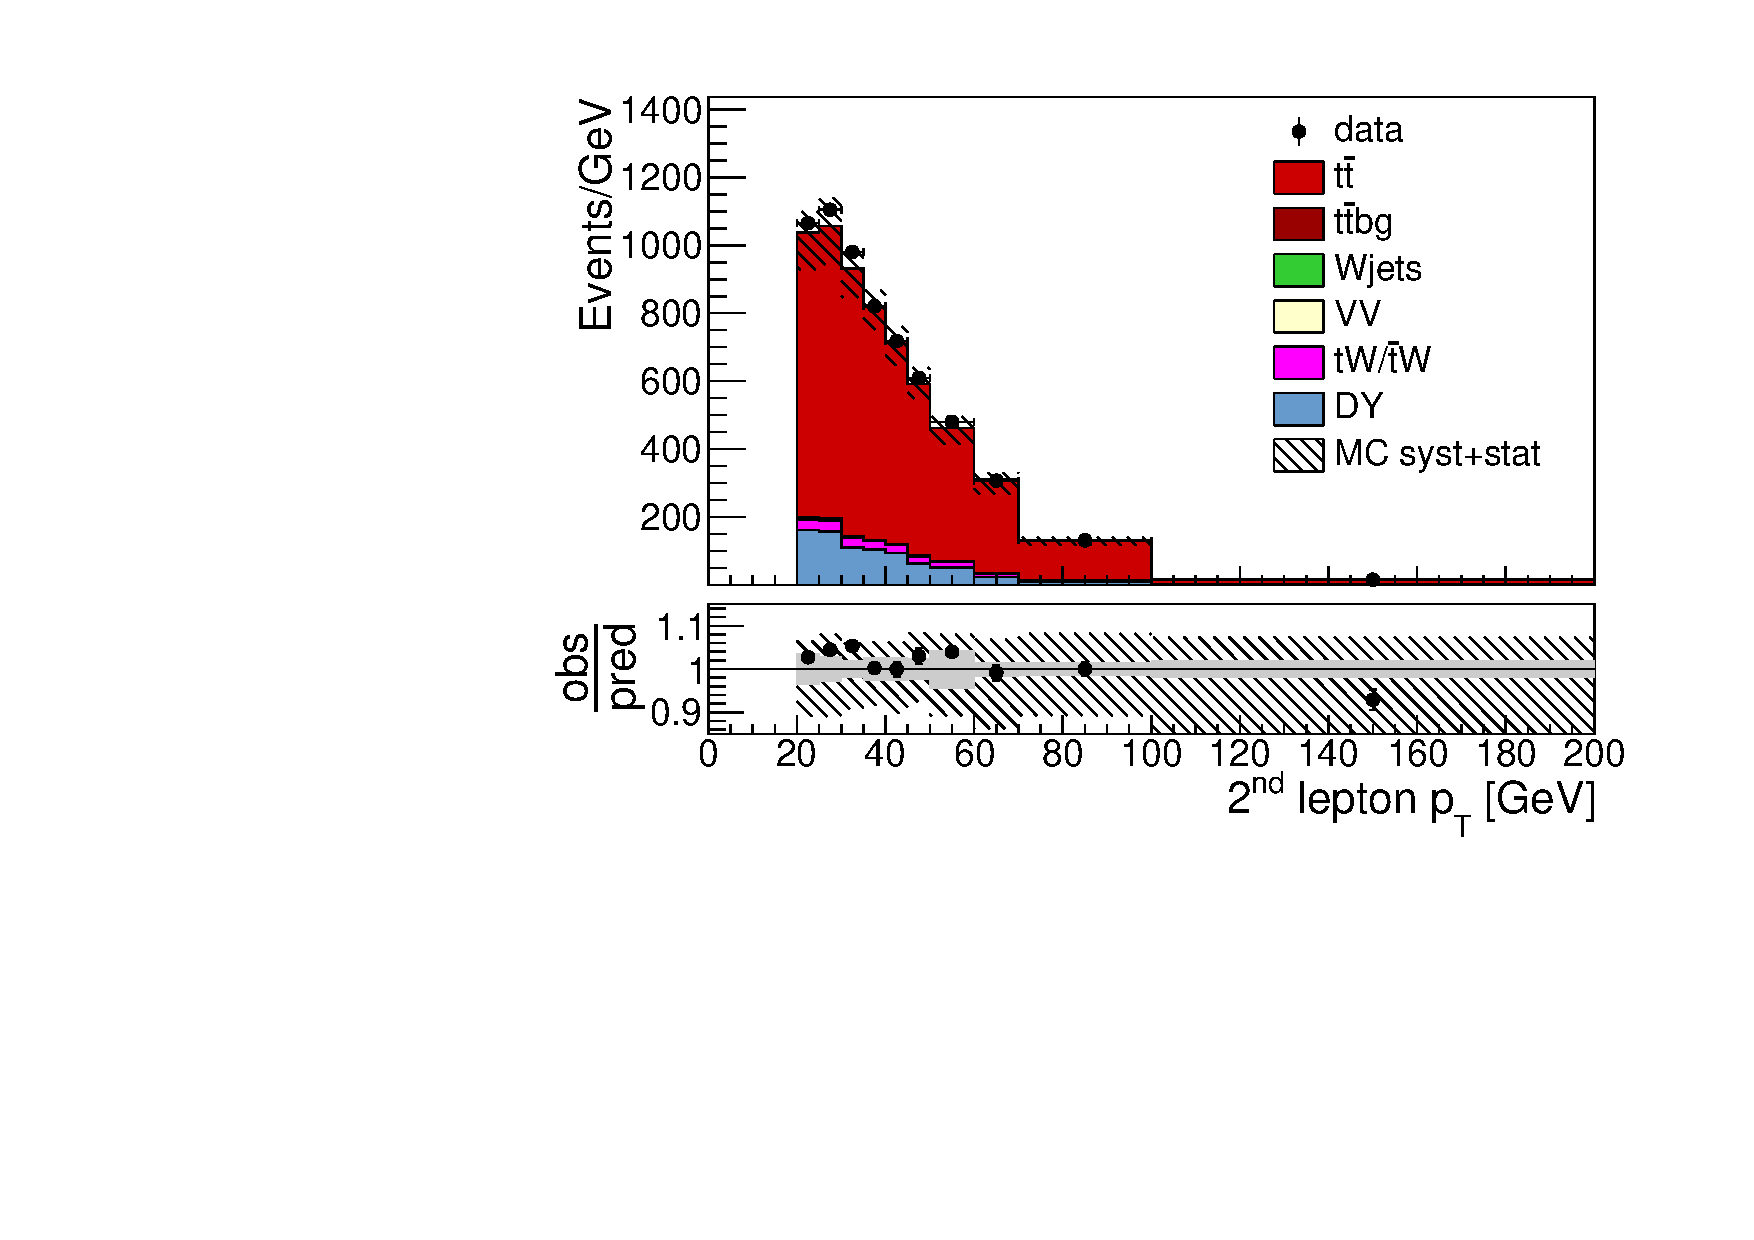
\includegraphics{CrossSection/Figures/ControlPlots/ee_sysnom/seclead_lepton_pt_step_8.pdf}}
    \resizebox{0.48 \textwidth}{!}{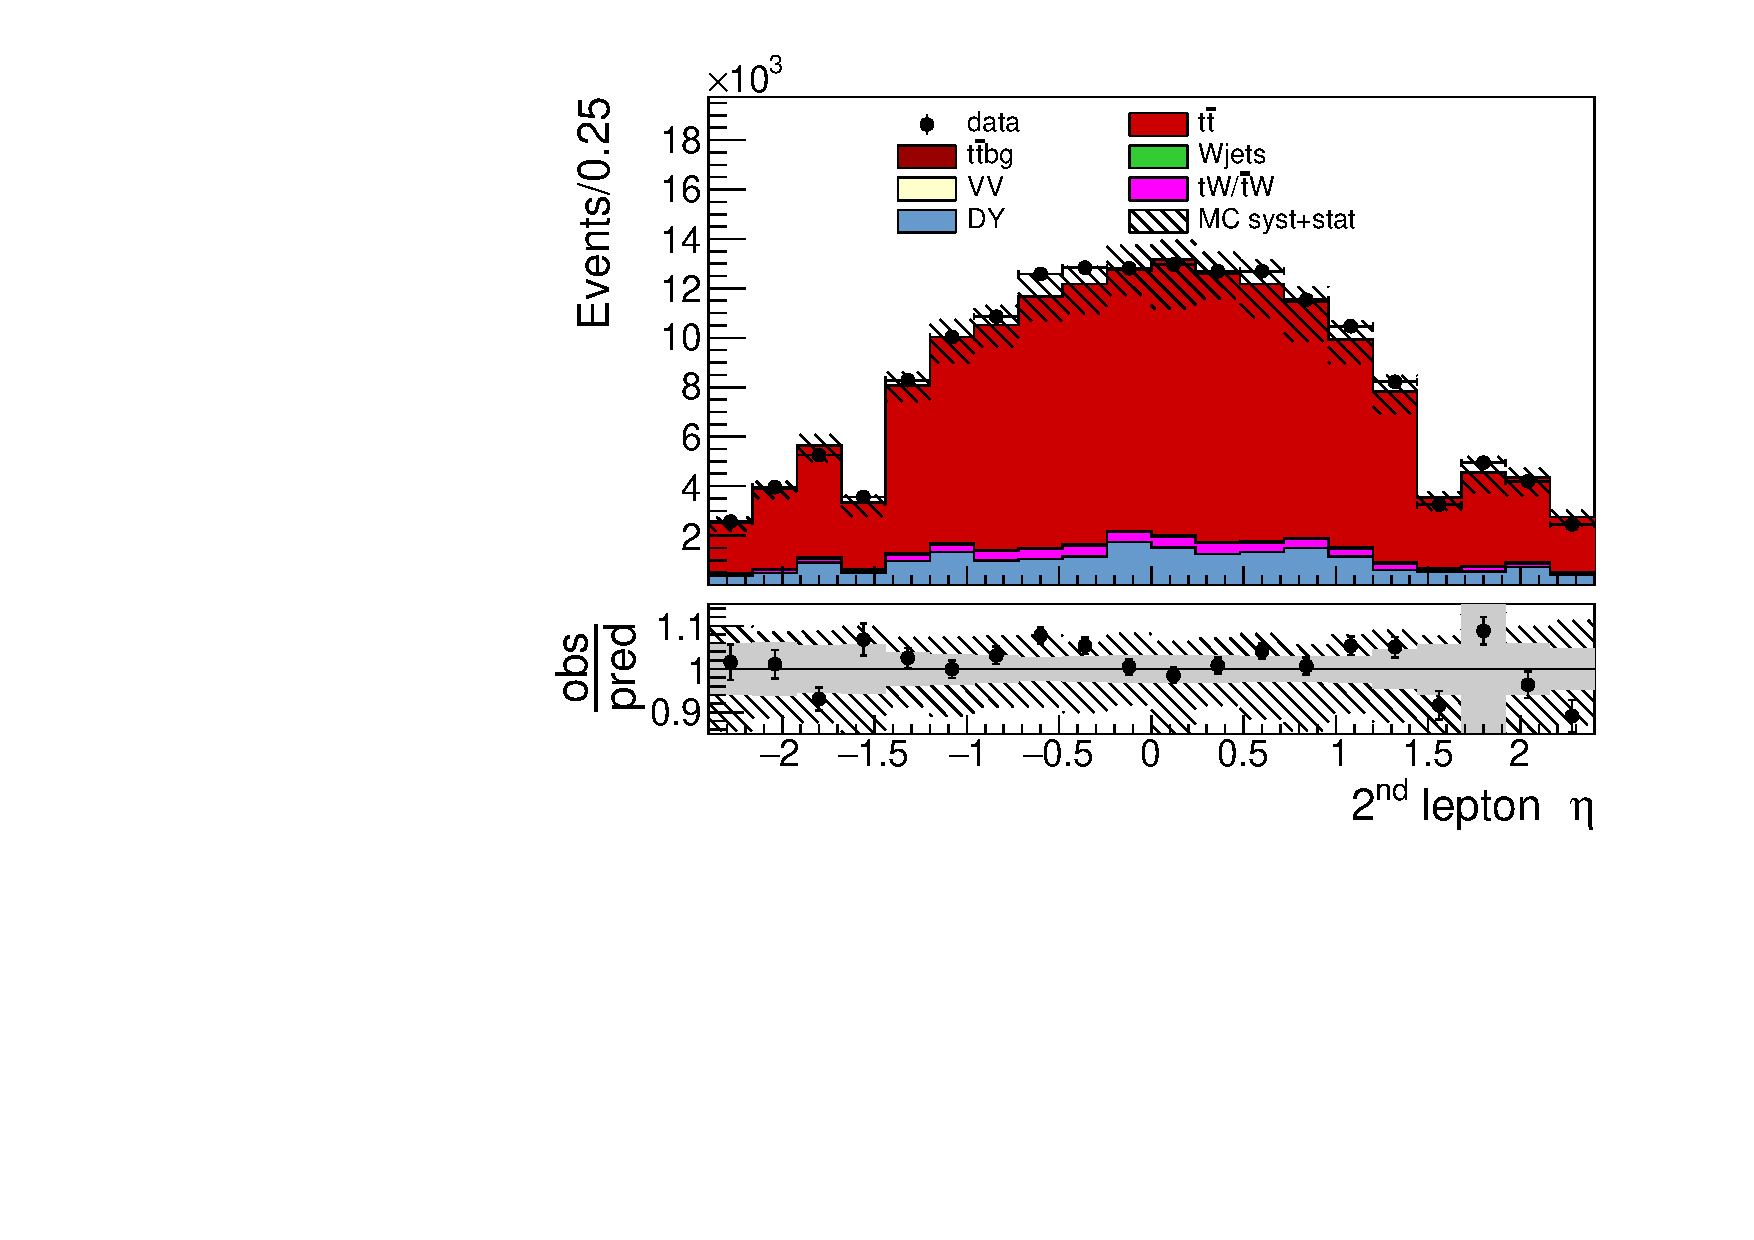
\includegraphics{CrossSection/Figures/ControlPlots/ee_sysnom/seclead_lepton_eta_step_8.pdf}}
    \resizebox{0.48 \textwidth}{!}{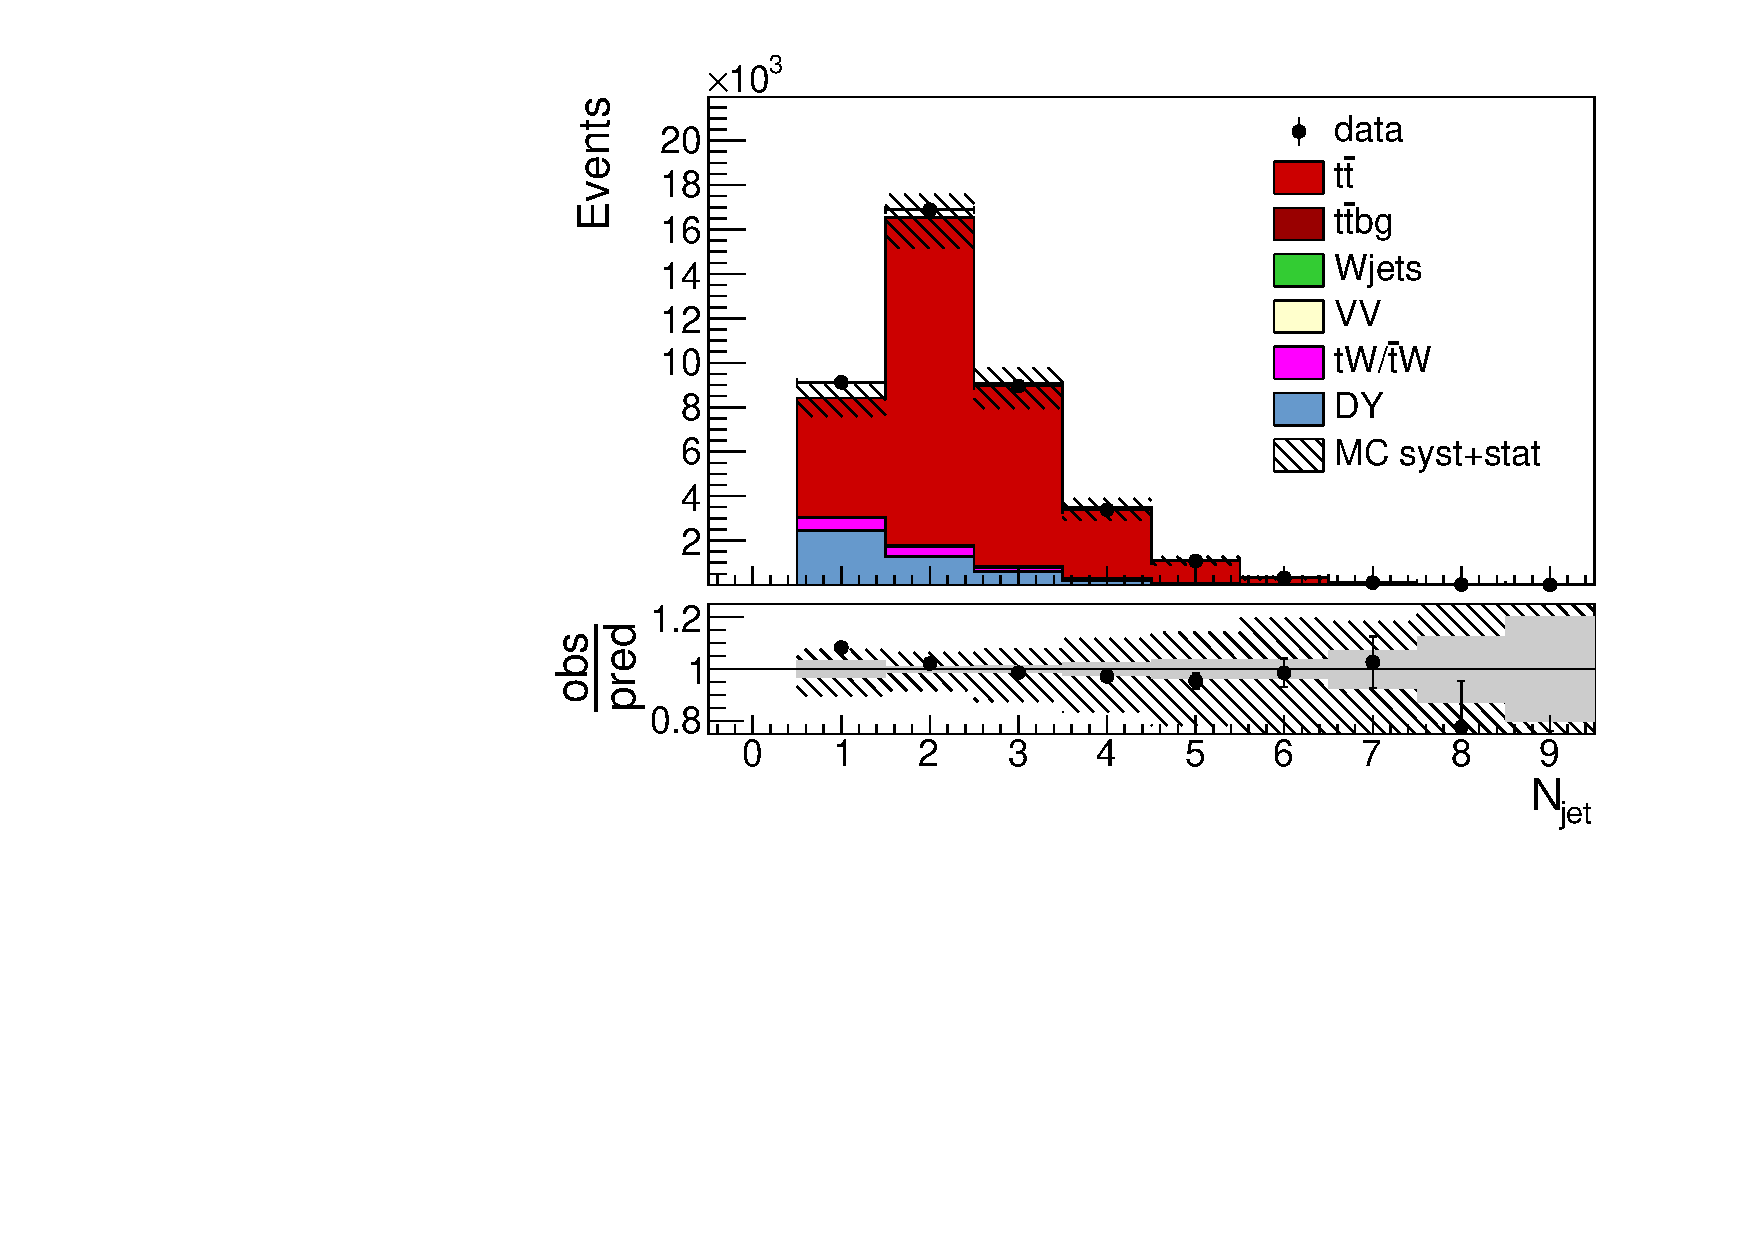
\includegraphics{CrossSection/Figures/ControlPlots/ee_sysnom/selected_jets_multi_step_8.pdf}}
    \resizebox{0.48 \textwidth}{!}{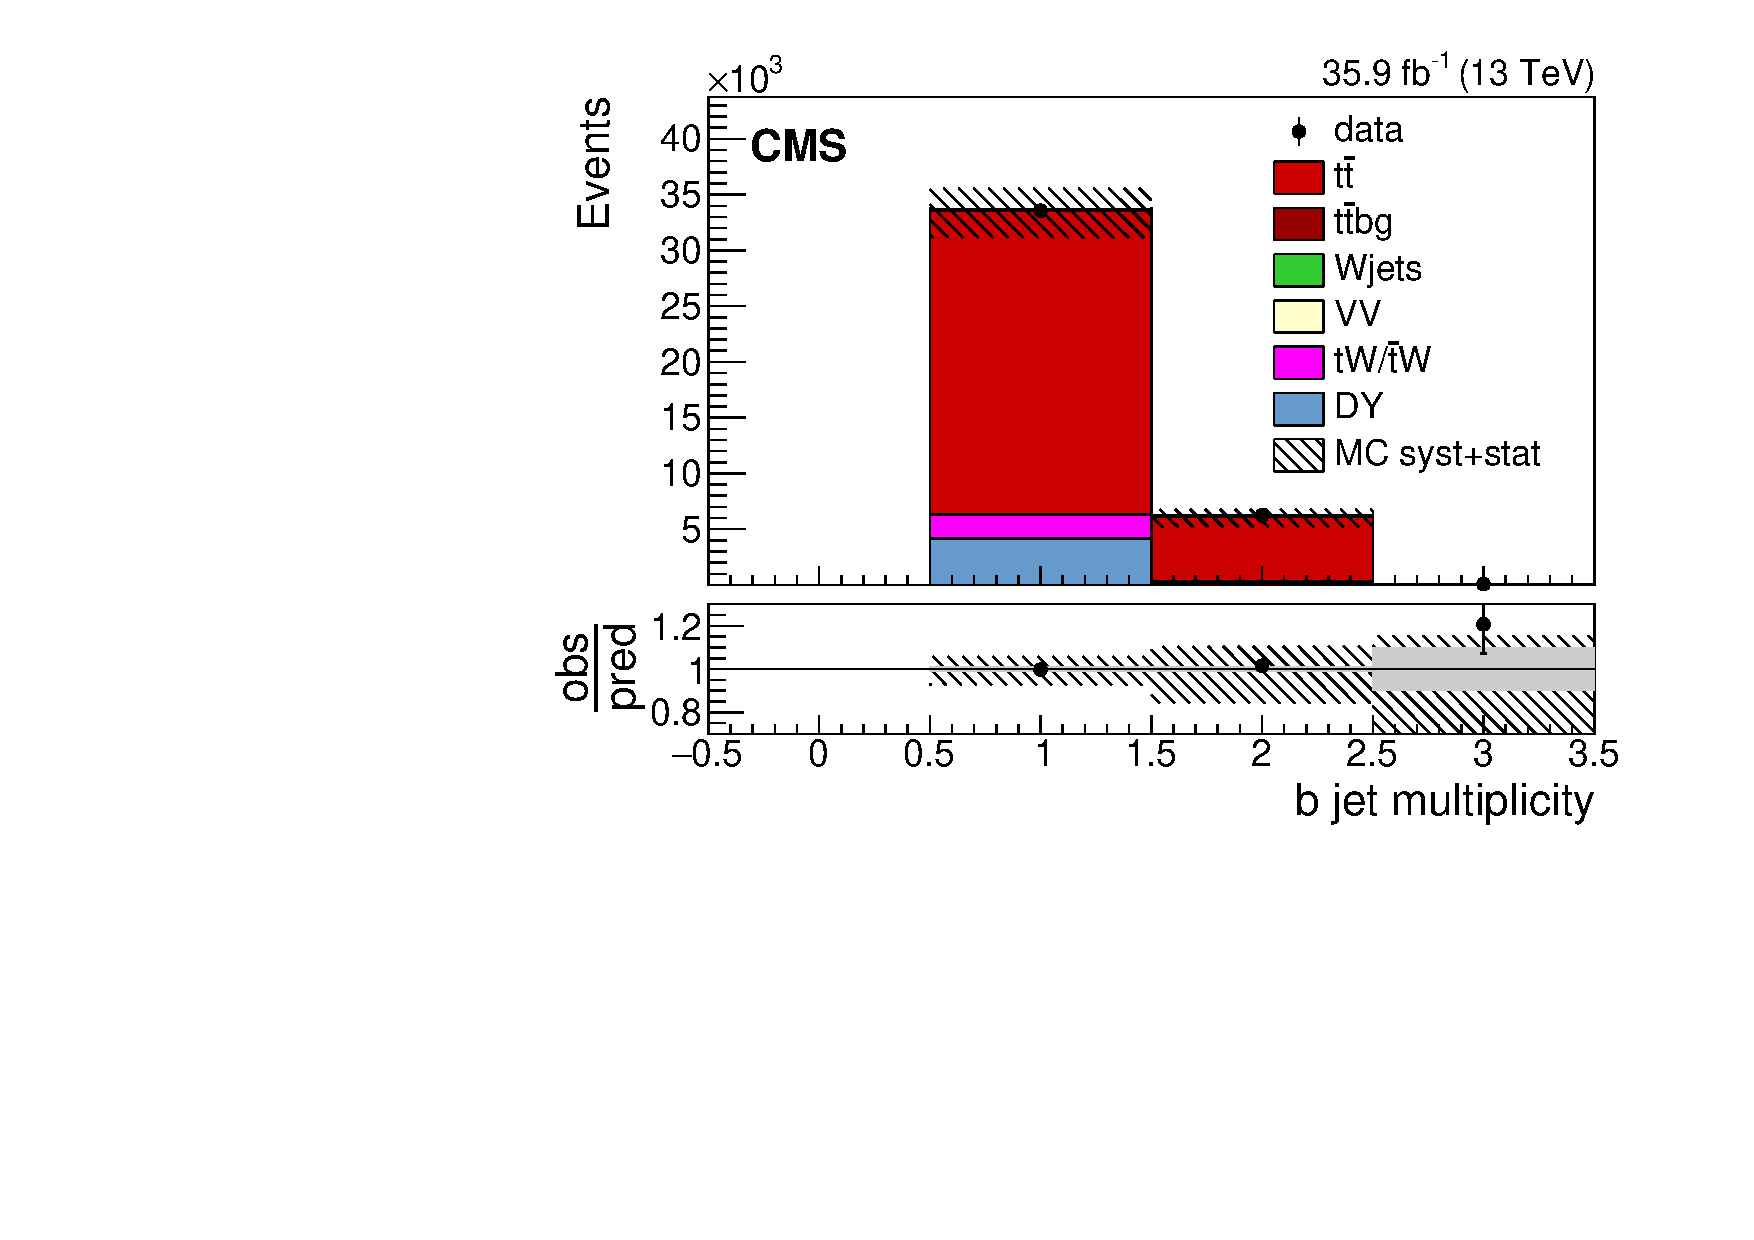
\includegraphics{CrossSection/Figures/ControlPlots/ee_sysnom/selected_b-jet_multi_step_8.pdf}}
      \caption{Transverse momentum (left) and pseudorapidity (right)
        of leading (first row) and second-leading (second row) lepton in the \ee channel after the
        event selection required by the \ttbar cross section
        extraction technique based on a simultaneous fit. Jet and b-jet multiplicity after the same selection steps are
        shown in the third row. The hatched
        bands correspond to the total uncertainty on the sum of the
        predicted yields. 
        %agrohsje , excluding luminosity and background
        %normalization uncertainties. 
        The ratios of data to the sum of the predicted yields are
        shown at the bottom of each plot. Here, the solid gray band
        represents the contribution of the statistical uncertainty.}  
       \label{fig:xsec_ee_ctrplots}
  \end{center}
\end{figure}

As described in Section \todo{Ref to reconstruction} the efficiency for the reconstruction of physics objects is different in data and simulation. This difference needs to be corrected in simulation.
This is especially important for leptons since we require two of those in the selection.
In order to assess the quality of the correction a carefull look into sensitive variables is important. Any large discrepancies between simulation and prediction would suggest that these corrections
are not optimal for the given selection.
The invariant mass of the dilepton system is shown in Figure \ref{fig:xsec_ctrplots_mll} for all three decay channels and depending on the number of b-tagged jets.
The simulation agrees with the measurement, so it can be assumed that the efficiency corrections are accurate.
The figures also show again how the DY contribution decreases when more b-tagged jets are required.


\begin{figure}[htbp!]
  \begin{center}
    \resizebox{0.48 \textwidth}{!}{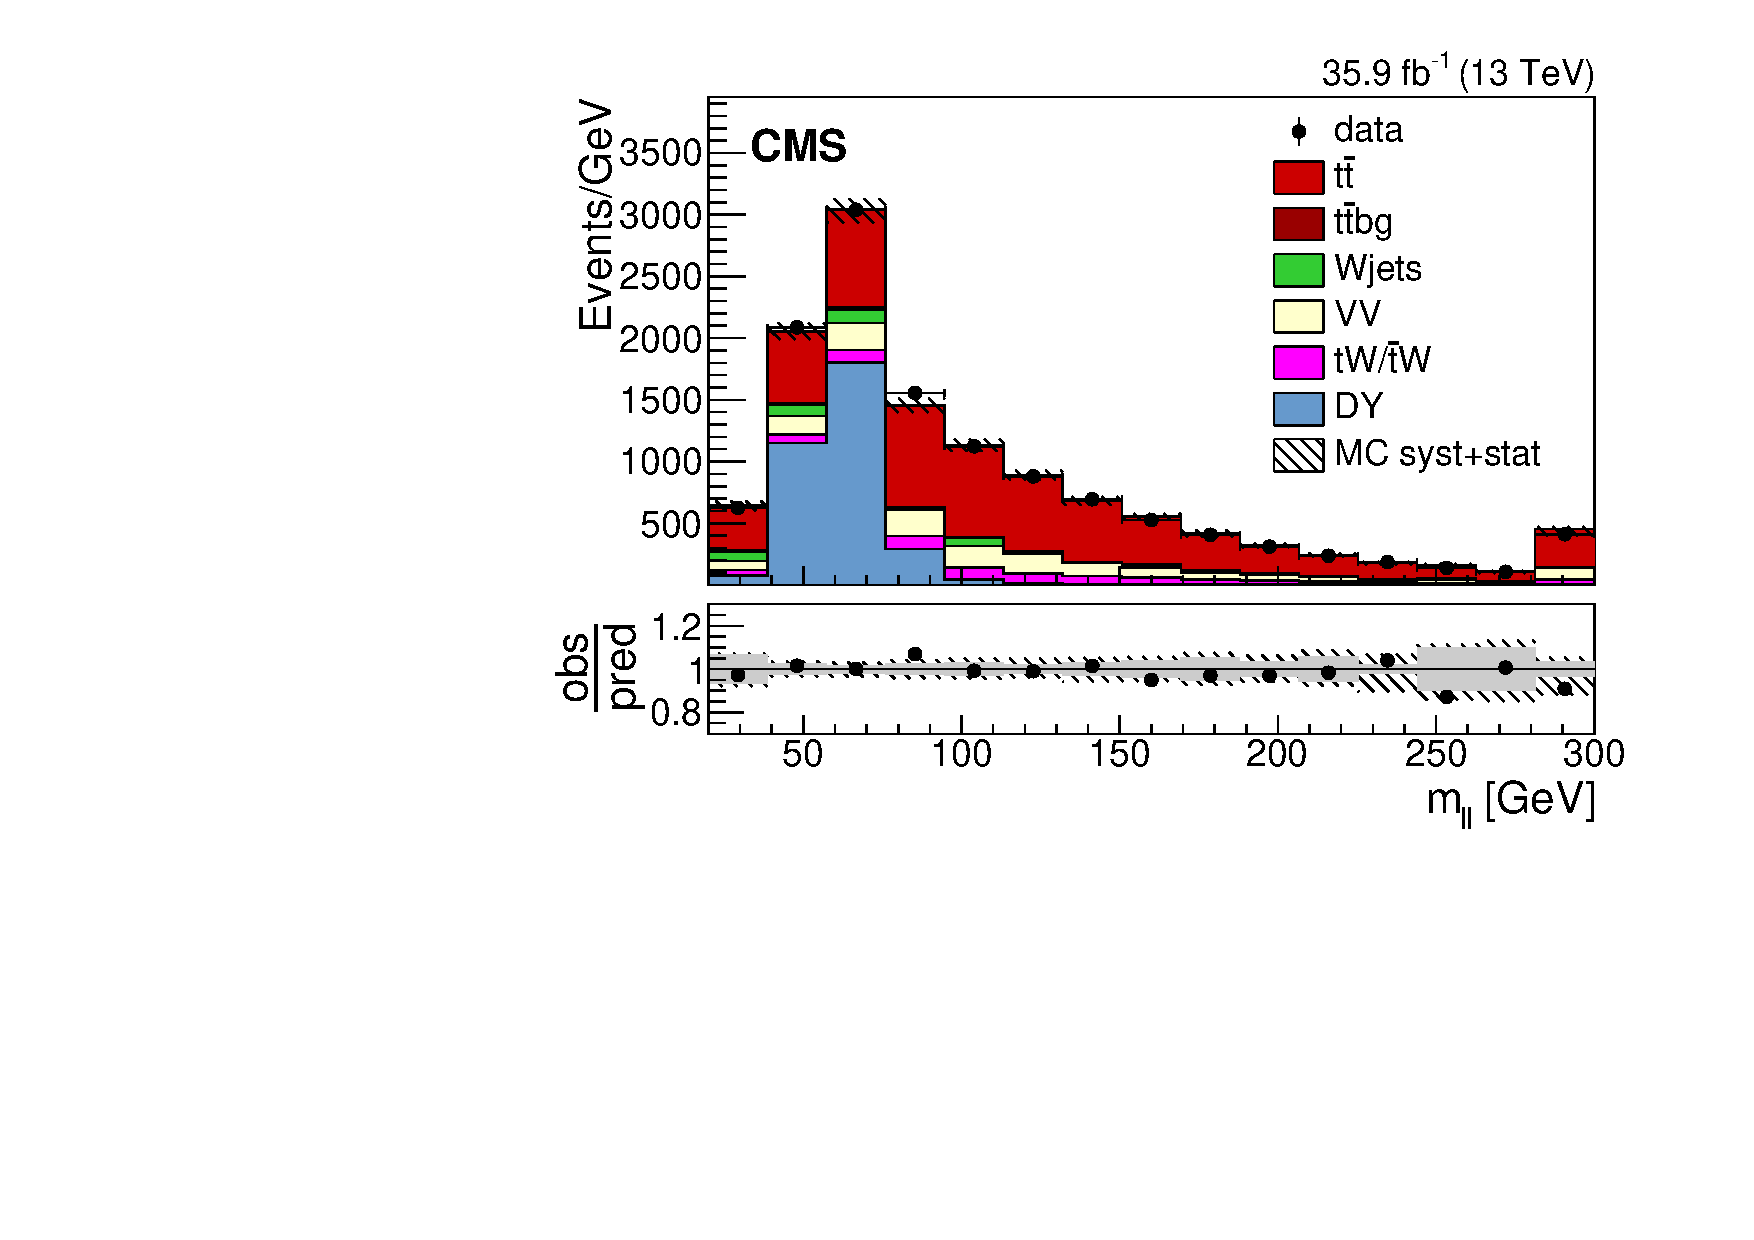
\includegraphics{CrossSection/Figures/ControlPlots/emu_sysnom/mll_0_b-jets_step_8.pdf}}
    \resizebox{0.48 \textwidth}{!}{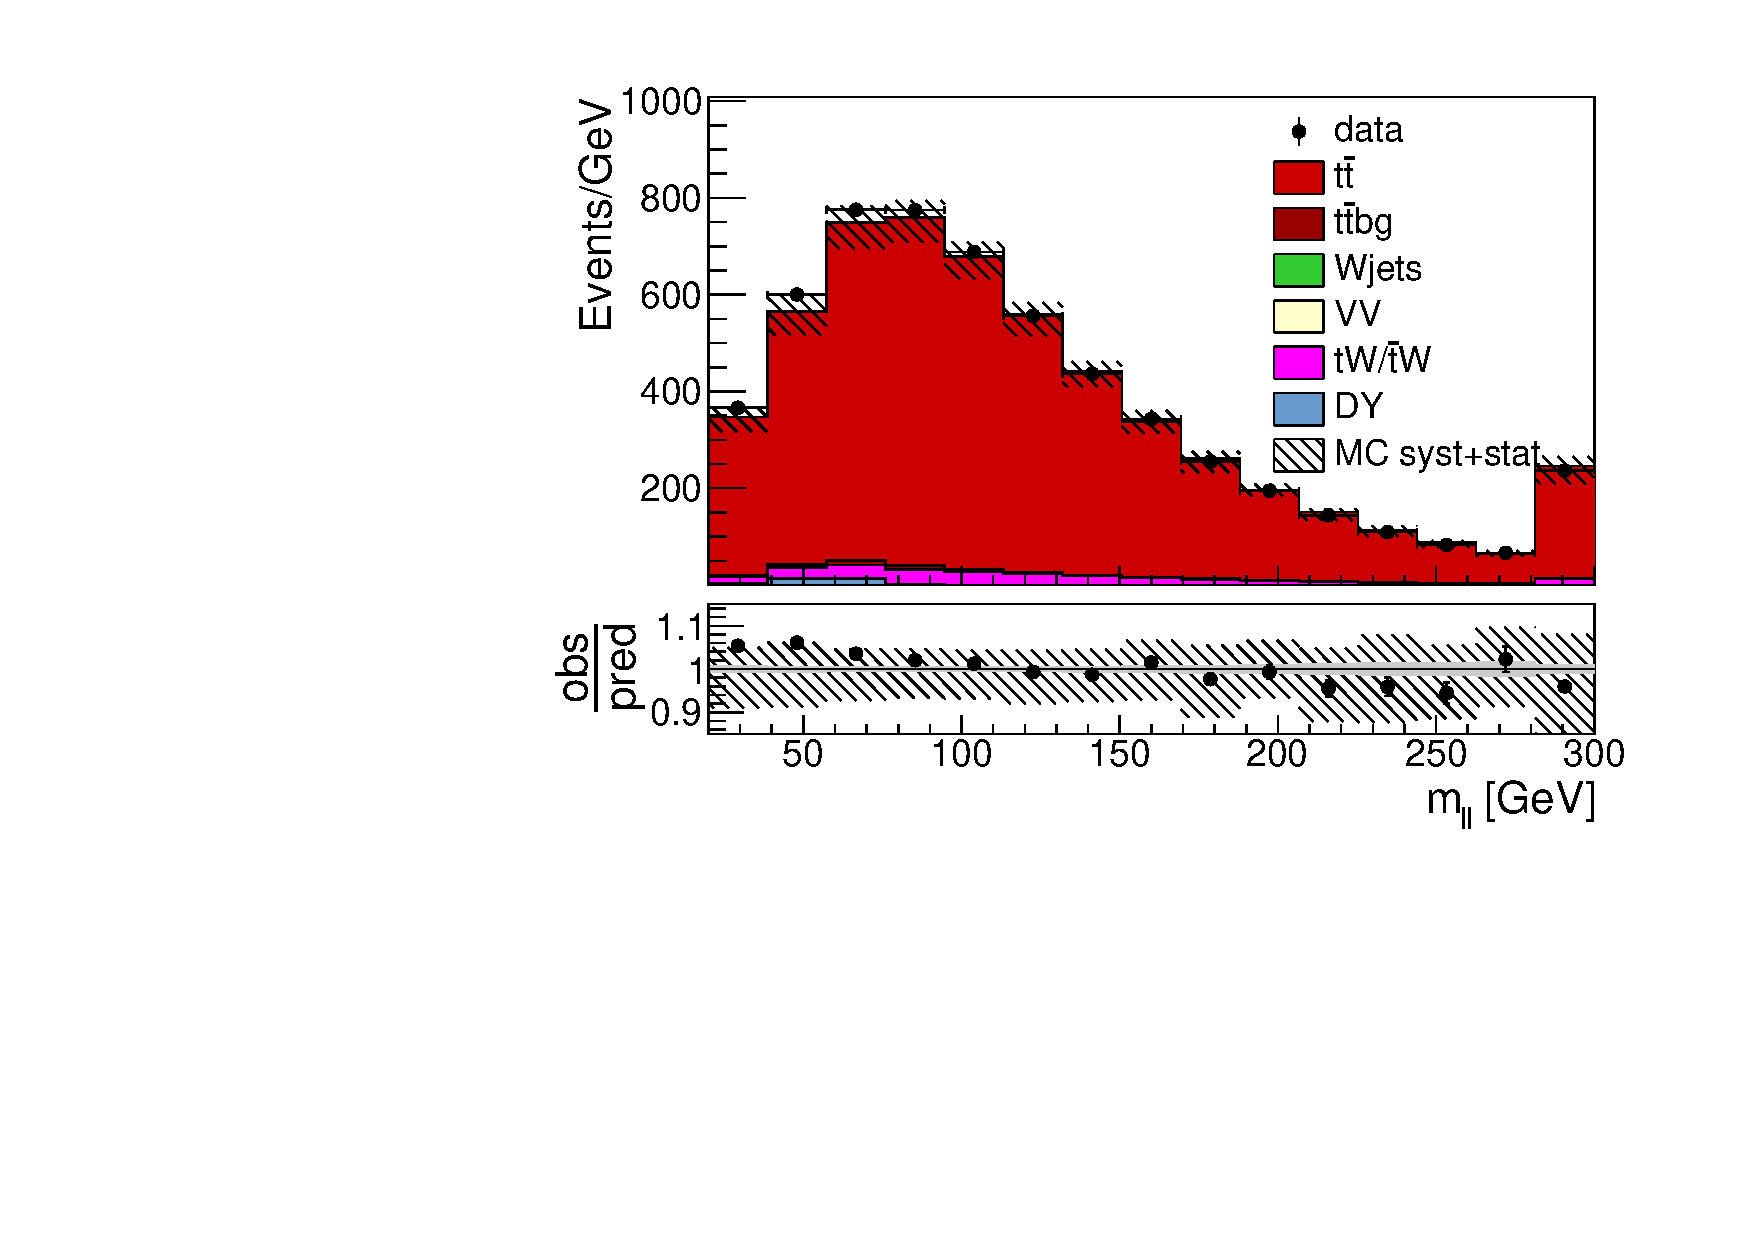
\includegraphics{CrossSection/Figures/ControlPlots/emu_sysnom/mll_1_b-jets_step_8.pdf}}
    \resizebox{0.48 \textwidth}{!}{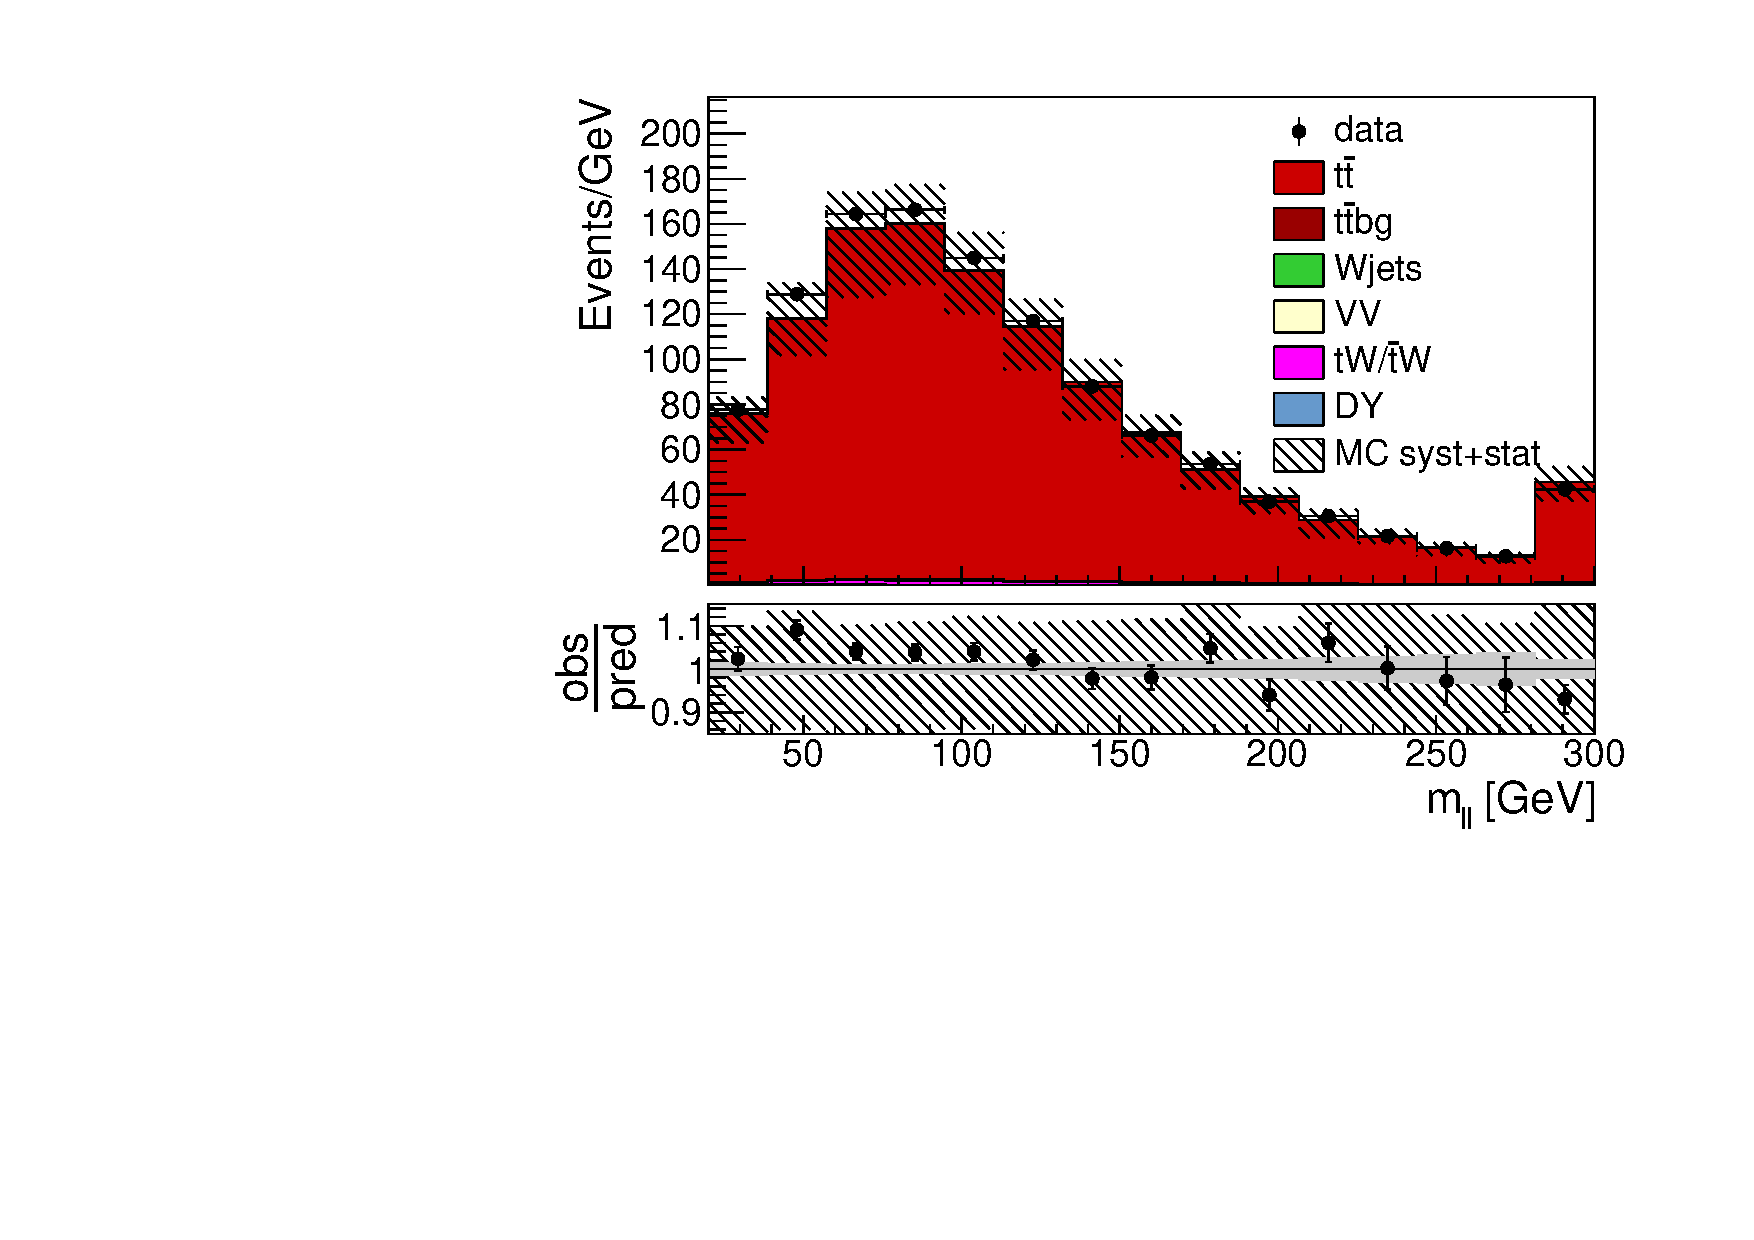
\includegraphics{CrossSection/Figures/ControlPlots/emu_sysnom/mll_2_b-jets_step_8.pdf}} \\
        \resizebox{0.48 \textwidth}{!}{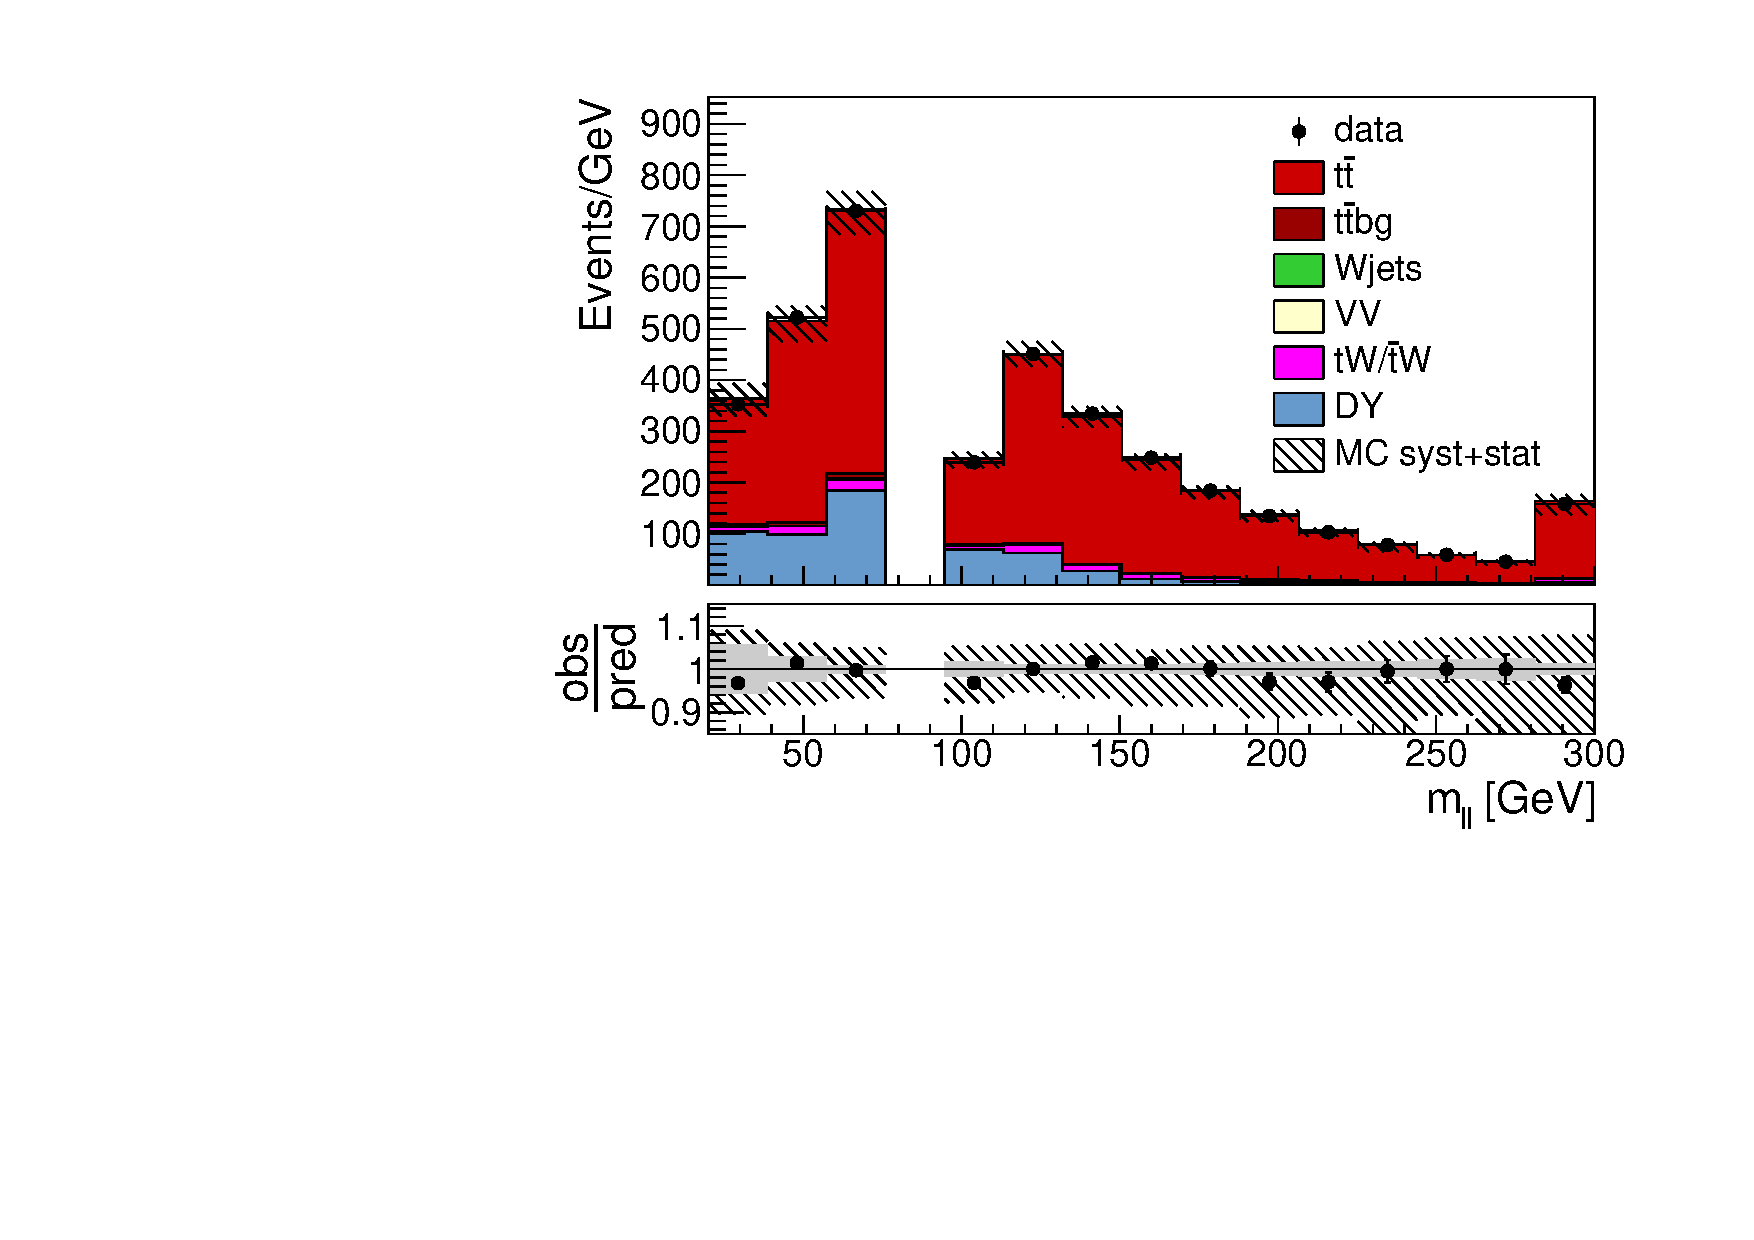
\includegraphics{CrossSection/Figures/ControlPlots/mumu_sysnom/mll_1_b-jets_step_8.pdf}}
    \resizebox{0.48 \textwidth}{!}{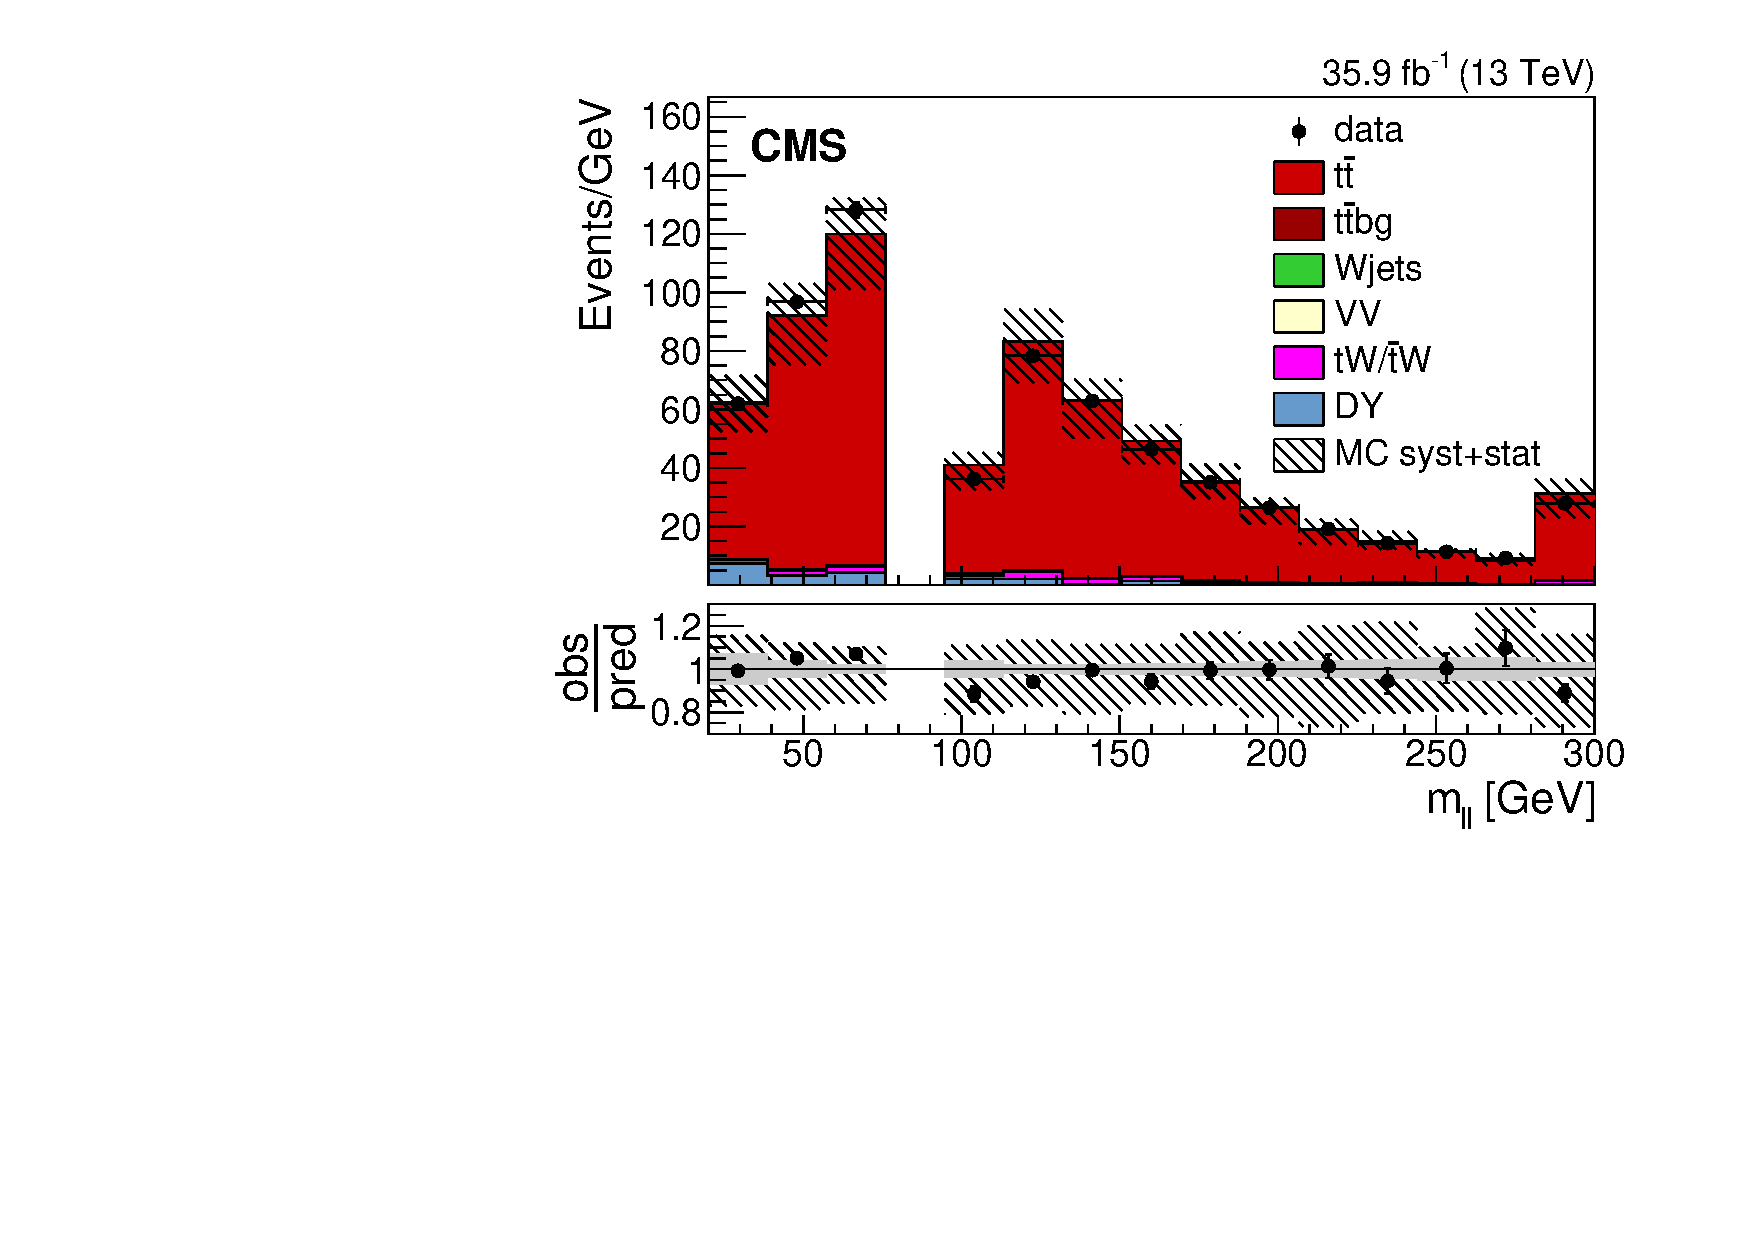
\includegraphics{CrossSection/Figures/ControlPlots/mumu_sysnom/mll_2_b-jets_step_8.pdf}} \\
        \resizebox{0.48 \textwidth}{!}{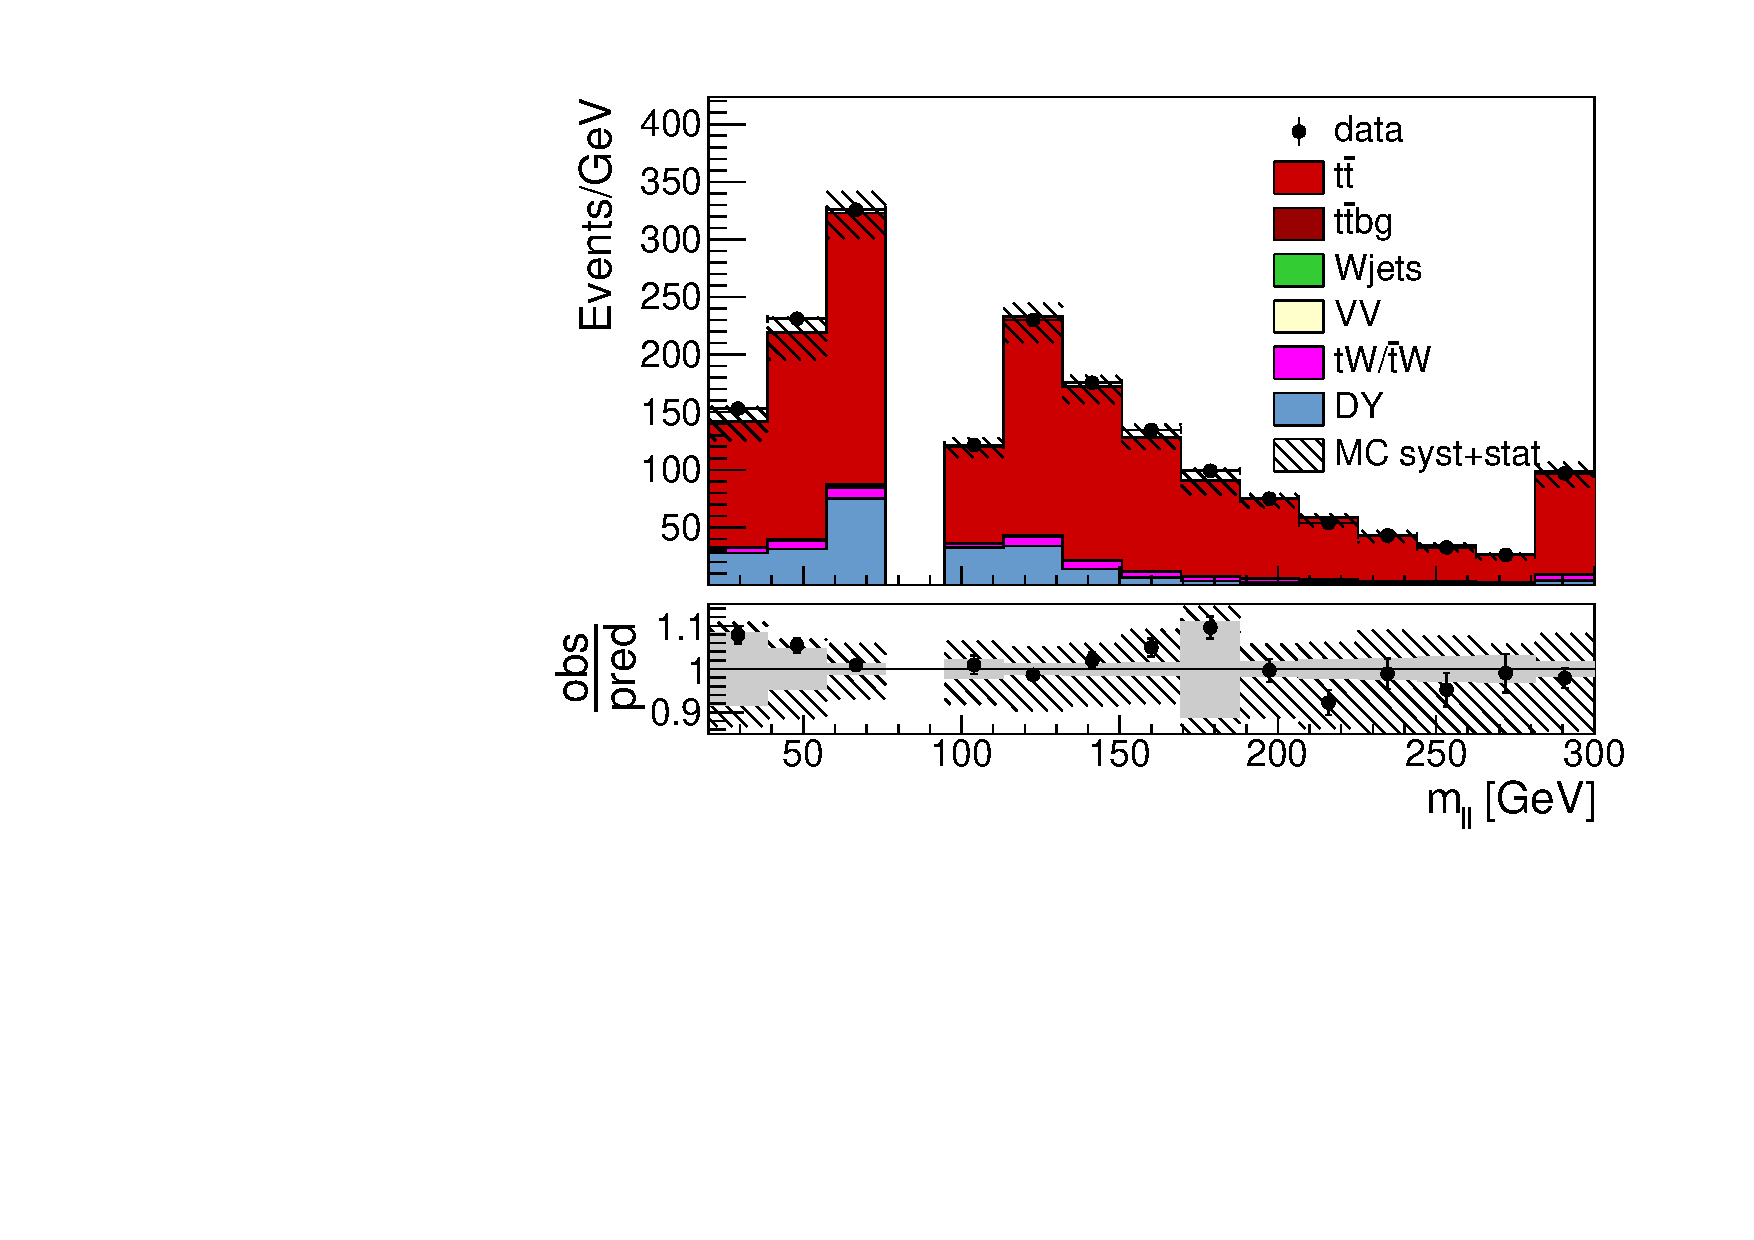
\includegraphics{CrossSection/Figures/ControlPlots/ee_sysnom/mll_1_b-jets_step_8.pdf}}
    \resizebox{0.48 \textwidth}{!}{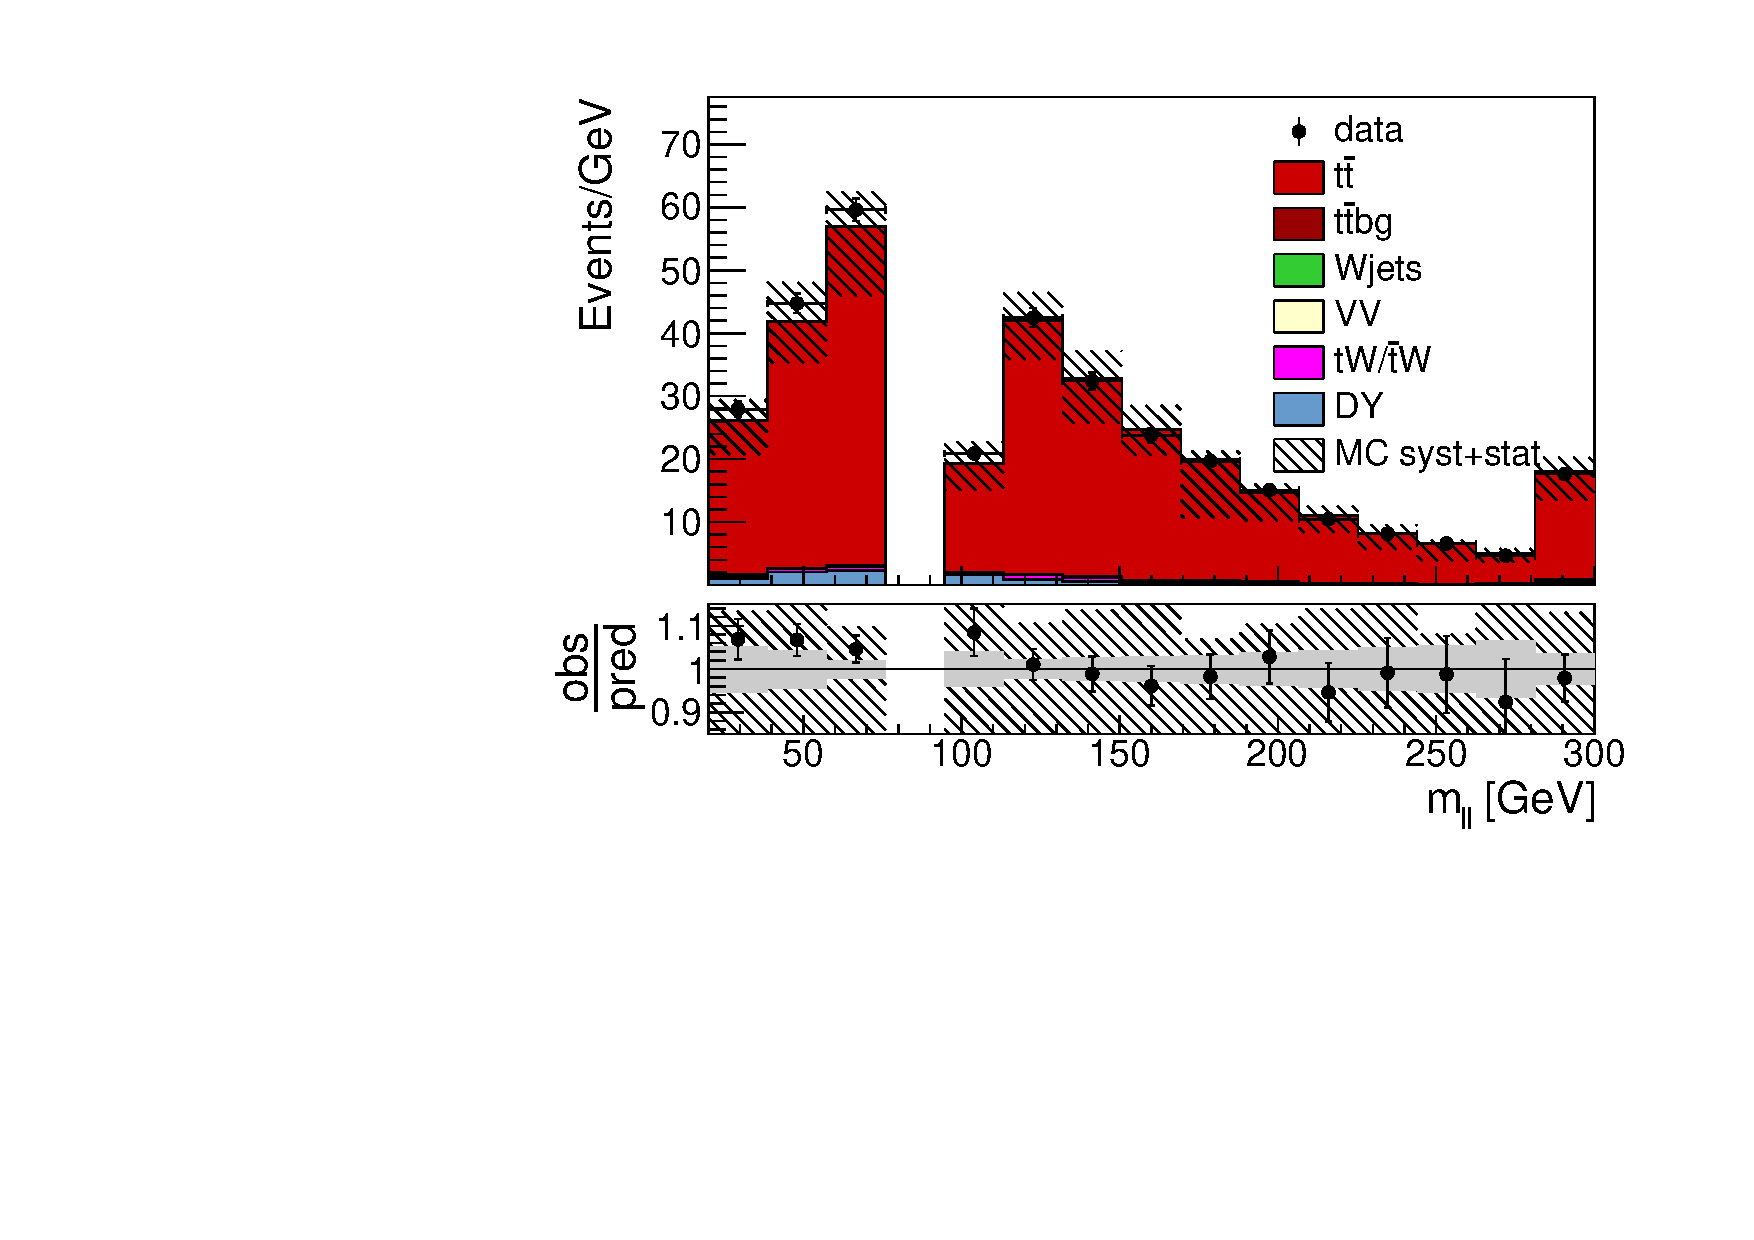
\includegraphics{CrossSection/Figures/ControlPlots/ee_sysnom/mll_2_b-jets_step_8.pdf}}

      \caption{Invariant mass of the dilepton system with zero (top row left), one (top row right) and two (second row) b-tagged 
      jets in the \emu channel. The invariant mass of the dilepton system in the \mumu (third row) and \ee (bottom row) with one (left)
      and two b-tagged jets (right).
        %agrohsje , excluding luminosity and background
        %normalization uncertainties. 
        The ratios of data to the sum of the predicted yields are
        shown at the bottom of each plot. Here, the solid gray band
        represents the contribution of the statistical uncertainty.}  
       \label{fig:xsec_ctrplots_mll}
  \end{center}
\end{figure}






